\documentclass{book} % utf8,utf8x
%\usepackage[utf8]{inputenc}

\usepackage{mystyle} 
\usepackage{customcolors}
\usepackage{mycommands}
\makeindex

% Title
\title{Python for Data Analysis \\ \scalebox{0.8}{Lecture Notes}}


\author{\scalebox{1}{By: \link{https://github.com/alexanderthclark}{Alexander Clark}\thanks{\texttt{ac4725@columbia.edu}\hspace{2pt}\faHandPeaceO}} \\
 {\scalebox{0.8}{\centering\emph{Columbia University SPS}}} }

\vspace{4cm}

\date{\scalebox{.8}{This version: \today}}

% name the list of listings 
\renewcommand\lstlistlistingname{Code} 
%\setcounter{tocdepth}{1}

\begin{document}

\frontmatter
\maketitle


\vfill 
%% State your copyright details as desired. 
% You might instead use the doclicense package 
% https://ctan.org/pkg/doclicense?lang=en
% Then simply add \doclicenseThis

Copyright Informatation Here. 



%\doclicenseThis

\vspace{5cm}

%\vfill
%\thispagestyle{empty}

\tableofcontents
%% Add list of listings for code
%\lstlistoflistings

\newpage

% I use * to make these unnumbered and then manually add to the toc

\chapter*{Preface}
\addcontentsline{toc}{chapter}{Preface}
\markboth{}{Preface}
These are my lecture notes for Python for Data Analysis, which I consider a work in progress. They're not written to replace class attendance, so you might not find them self-contained. 

The main references for these notes are \cite{lubanovic2019introducing} and \cite{vanderplas2016python}. There are many other fantastic books and resources for self-studying Python. I encourage you to find as many supplementary sources as you find helpful, but to return to these notes to help focus on what will be important for doing well on assignments and exams in this course. 

I've seen this material presented in many different orders. What seems unavoidable in any bearable introduction to Python is that some concept might be slipped in informally before we regroup for a formal explanation of how some data type works or why we keep using words like \emph{object}, \emph{method}, or \emph{callable}. This isn't so different than learning a language through immersion. That's to say we'll be immersed and you might find yourself flipping backwards or forwards in these notes. You could also compare it to bulking and cutting in bodybuilding. Let me know if you see anything that could use restructuring.  

Famous mathematician Paul Halmos counseled students not to study math passively. With Python, this is also good advice. Ease into the language, but don't remain satisfied with running others' code or making only minimal edits. Work from scratch and relish the detours. 

\begin{center}
\href{https://abstrusegoose.com/353}{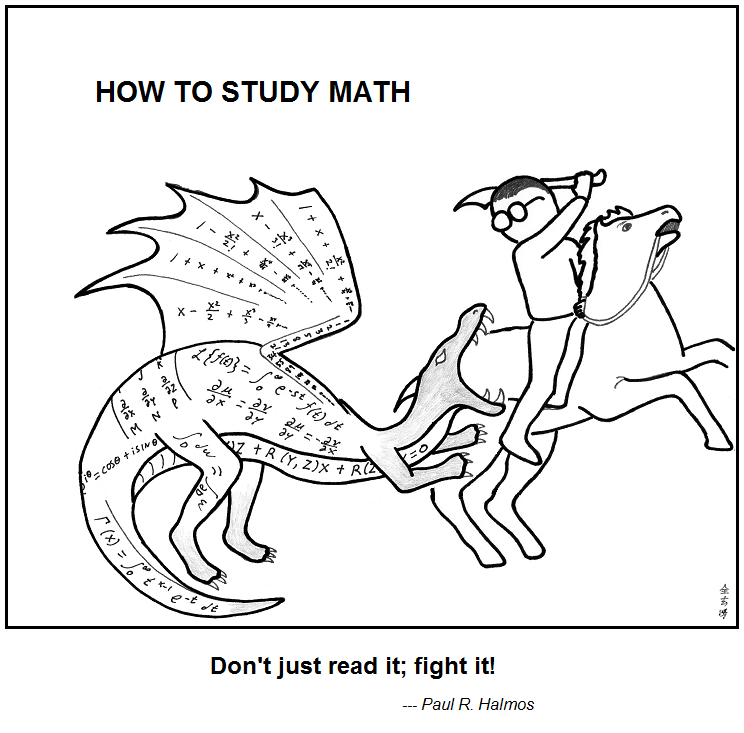
\includegraphics[width = .51\textwidth]{HowMath.png}}

\vspace{-14pt}
\scalebox{0.6}{Source: \link{https://abstrusegoose.com/353}{AbstruseGoose.com}}
\end{center}

\mainmatter

% Part I --------------------------------
\part{Programming}

\chapter{Input, Processing, and Output}\label{chapter:c1}
%%% HELLO WORLD
\section{The Hello World Program}

To get started in any langauge, printing ``Hello, World!'' might be the first step.\footnote{See
\link{https://en.wikipedia.org/wiki/\%22Hello,_World!\%22_program}
{the Wikipedia page for Hello, World.}}

\smallskip

In Python, we can print an input using the \lstinline[language = Python]{print()} function. We simply pass our
desired input within the parentheses, and Python will print the value.

 We can enter text as a \textbf{string}. Text entered inside single, double, or triple quotations is interpreted as a string.


\begin{lstlisting}[language = Python]
print('Hello, World')
print("Hello, World!")
print("""Hello,
World!""") \end{lstlisting}


\smallskip

In Python 2, the syntax would have been \lstinline[language = Python]{print 'Hello, World!'} without the parentheses. You shouldn't use Python 2 or bother learning its variations, but this is a good difference to understand. If you see this old syntax in an old Stack Exchange post or anywhere else, let that be a tipoff that you might be looking at Python 2 code, which might behave differently.

%%% Variables
\section{Variables}

A \textbf{variable} holds a value. It can be a string, a number, or perhaps a more complicated data type.
Variable assignment is done with the equals sign, \lstinline[language = Python]{=}.


\smallskip

\begin{lstlisting}
greeting = "Hello, World!"
my_favorite_number = 91
\end{lstlisting}

\smallskip

\noindent Now compare the output you get from the following.

\begin{lstlisting}
print(greeting)
print('greeting')
print("Hello, World!")
print(91)
print(my_favorite_number)
print('my_favorite_number')
print("My favorite number is", my_favorite_number)
print("My favorite number is ", my_favorite_number)
\end{lstlisting}


\smallskip

PEP 8 addresses variable names \textcolor{blue}{\href{https://www.python.org/dev/peps/pep-0008/\#function-and-variable-names}{here}}.
Use lowercase and underscores. This is good advice, but I don't see any reason to be too wedded to this. If you want to assign a matrix to a variable, 
it's reasonable to use an uppercase letter as the variable name. There, a math convention overrides a Python convention. %Indeed, Gaddis is fine with uppercase (p. 43).

\smallskip

More importantly, avoid Python key words in your variable names. \textcolor{blue}{\href{https://www.w3schools.com/python/python_ref_keywords.asp}
{Here}} is a list of key words which have a specific meaning in code. See \cite{lubanovic2019introducing} page 27 for a complete list of rules for variable names. An IDE or code editor will make this easier for you by highlighting keywords that you shouldn't use for variable names. 

\begin{center}
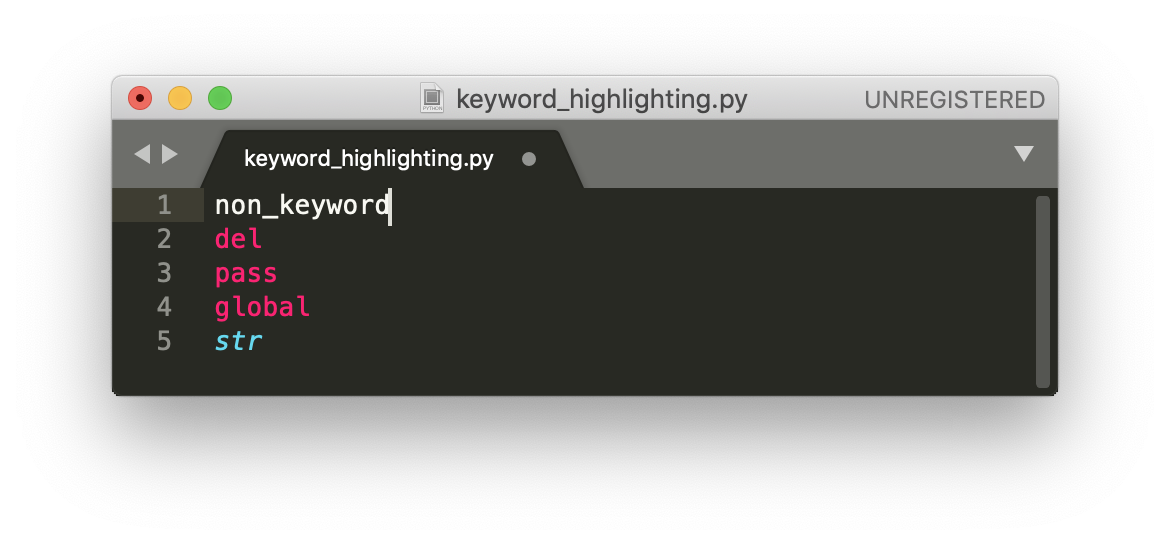
\includegraphics[width = .53\textwidth]{images/sublime_keyword_highlight.png}
\end{center}

While you simply can't assign any value to \code{class}, you can assign a value to \code{str}. Even though it's permitted, I would suggest you never assign a value to \code{str} because it can be used to confirm something is a string type. The same goes for keywords like \code{int}. Consider the program below. 

\begin{lstlisting}
s = 'Python'
is_string = type(s) == str
\end{lstlisting}

The above works so that \code{is_string} holds a value \code{True} if and only if \code{s} is a string. In this case, \code{is_string = True} The program below also runs, but it does something different. \code{str} holds the value \code{10} so the last line checks if the type of \code{s} is equal to ten. Now, \code{is_string} holds the value \code{False}.

\begin{lstlisting}
s = 'Python'
str = 10
is_string = type(s) == str
\end{lstlisting}


Finally, consider how the variables chapter in \cite{lubanovic2019introducing} opens with a quote from \link{https://www.biblegateway.com/passage/?search=Proverbs\%2022\%3A1&version=NRSV}{Proverbs 22:1}. ``A good name is rather to be chosen than great riches.'' In its Biblical context, this expresses the idea that a good reputation is better than money and that the name is an expression of the inner character of its bearer. \cite{lubanovic2019introducing} is stressing the importance of variable names in a different way. Well-named variables help the reader and user of your code. In a way, instead of indicating the character of the person, variable names actually shape the character of your code. Be thoughtful of this, so if you're using \code{n} for the number of apples, perhaps you can spare the keystrokes for \code{num_apples}. We might complete the Biblical analogy by saying that readable code with well-named variables is better than confusing code that might run faster or have been written faster. This concern for readability brings us to our next topic, comments. 


\section{Comments}
\noindent \textit{Comments are briefly addressed in \cite{lubanovic2019introducing} Chapter 4.}

Commenting your code is helpful if you care about your colleagues or your future self. Comments should add clarity to
the intention and workings of code. A comment is a piece of code that isn't actually executed---it's a comment left for the reader or the person who inherits and modifies your code.
Everything after a \lstinline[language = Python]{#} will be ignored by the Python interpreter.

\begin{lstlisting}[language = Python]
# This will print a greeting.
print('Hello, World!') \end{lstlisting}

\smallskip
 You might also use end-line comments like the following

\begin{lstlisting}[language = Python]
print('Hello, World!') # Prints a greeting \end{lstlisting}

\smallskip

 PEP 8 addresses comments \textcolor{blue}{\href{https://www.python.org/dev/peps/pep-0008/\#comments}{here}}.
I don't intend to grade based on the stylistic orthodoxy of your comments, but spaces are free so I do recommend 
\lstinline[language = Python]{# Comments like this} instead of \lstinline[language = Python]{#Comments like this}.

Perfect comment technique does not correct for bad code though. Compare the following blocks of code. 

\begin{lstlisting}
x = 90 # Wins
y = 10 # Losses
z = x/y # Win Loss Ratio
a = 100 * x/(y+x) # Winning Percentage
\end{lstlisting}

\begin{lstlisting}
wins = 90
lossses = 10
win_loss_ratio = wins/losses
winning_percentage = 100 * wins / (losses + wins)
\end{lstlisting}

The first block is commented and the second is not. Still, the second code block is much better because the variable names are chosen so you don't \emph{need} comments. Good naming becomes even more important as the program becomes longer and the variable is used over and over. See also the discussion in \cite{long2021}.



\section{Data Types and Conversion}

To start, we are concerned with strings, integers, and floats. In Python, these are classes 
\lstinline{str}, \lstinline{int}, and \lstinline{float}.
You can check the type of variable or value using \code{type()}.


\begin{lstlisting}[language = Python]
string_example = ''
int_example = -1
float_example = -1. \end{lstlisting}

\smallskip
 Some types can be converted by using \lstinline[language = Python]{str()},
\lstinline[language = Python]{int()}, or \lstinline[language = Python]{float()}. You might informally call these functions, but they actually aren't because function has a special meaning that's reserved for other things. We'll call them callables, which is a more general category. 


\begin{lstlisting}
print(type(1))
print(type(str(1)))
\end{lstlisting}

\section{Input}

It's not that common for a data science workflow, but you can read input using \lstinline[language = Python]{input()}.
The input is always read in as a string.

\begin{lstlisting}[language = Python]
favorte_color = input("What is your favorite color?")
favorite_number = input("What is your favorite number?")
attending_in_person = input("I am attending class in person.") \end{lstlisting}


\section{Calculations}

You can use Python as a calculator. Below is the list of operations and symbols. 

\begin{center}
{\setlength{\tabcolsep}{2em}
\begin{tabular}{lll}
\toprule
Operator & Description \\
\midrule
\code{+} &    Addition \\
\code{-} & Subtraction \\
\code{*}  &    Multiplication \\
\code{/}  &   Floating point (normal) division \\
\code{//}  &  Integer (truncating) division \\
\code{\%} & Modulus (remainder) \\
\code{**} & Exponentiation \\
\bottomrule
\end{tabular}}
\end{center}


What might stand out is 
\begin{itemize}
\item Exponentiation is done with \lstinline[language = Python]{**}, not \lstinline[language = Python]{^}.
\item Integer division (rounds down) is done with \lstinline[language = Python]{//}.
\item The remainder of $x$ divided by $y$ can be found with \code{x \% y}, which might be read as
$x$ \emph{modulo} $y$. 
\end{itemize}

If a float is involved in an operation, the result will also be a float, as in \code{type(2 + 2.)}.


\chapter{If, Elif, Else}
\noindent \scalebox{1}{\textit{Reference: Lubanovic Chapter 4}}

Decision structures allow a program to have more than one path of execution. The path depends on condition.
The condition is either True or False, and so can be represented by a Boolean variable.

\section{If Statements}

Here's a joke. A programmer is going to the grocery store and his partner says, ``Buy a gallon of milk, and if there are eggs, buy a dozen.''
The programmer comes home with 13 gallons of milk.

\smallskip
\noindent Or consider the logical inference if you ask, ``Is it raining?'' and get a reply, ``Not hard.''


\begin{lstlisting}[language = Python]
if 2 + 2 > 4:
    print("Pigs can fly.")
    
if 2 + 2 == 4:
    print("Pigs cannot fly.")
    
if 'a' < 'b':
    print("It is true that 'a' is less than 'b'.")
    
if 'a' < 'A':
    print("It is true that 'a' is less than 'A'.")
    
if 'goon' == 'Goblin':
    print("A goon is a goblin.") \end{lstlisting}
    
%https://genius.com/annotations/2257/standalone_embed

If statements like the above rely on \emph{relational operators} (see Table 3-1 Gaddis p.112).

\begin{lstlisting}[language = Python]
if 2 == 2.:
    print("The integer and the float are equal.")
    
if 2 is 2.:
    print("The integer and the float are the same object in memory.") \end{lstlisting}

\section{If Elif Else Statements}

The natural counterpart to \code{if} is \code{else}. The code under \code{else} simply executes when the if condition is not satisfied. We also have \code{elif} (or else if) to help in the intermediate case, where we want another block of code to be run when the if condition is not satisified \emph{and} some other condition is satisfied.

Compare this program with a simpler version using else if conditions. 
\begin{lstlisting}
x = 1
if x == 0:
    print("zero")
else:
    if x < 0:
        print("negative")
        else:
            print("positive")
\end{lstlisting}


\begin{lstlisting}
x = 1
if x == 0:
    print("zero")
elif x < 0:
    print('negative')
else:
    print('positive')
\end{lstlisting}



Compare the output from the following programs.

\begin{lstlisting}[language = Python]
num = 0

if num < 1:
    print(num)
    num = num + 2
if num > 0:
    print(num, '!')
    num = num - 1000
if True:
    print(num, '?') \end{lstlisting}


\begin{lstlisting}[language = Python]
num = 0

if num < 1:
    print(num)
    num = num + 2
elif num > 0:
    print(num, '!')
    num = num - 1000
else:
    print(num, '?') \end{lstlisting}


\section{Logical Operators}

Suppose you want to execute some code if a number $x$ is between 10 and 20. You could use \emph{nested} if statements.
\begin{lstlisting}[language = Python]
x = 14
if x >= 10:
    if x <= 20:
        print("x is between 10 and 20.") \end{lstlisting}
        

\smallskip
\noindent But you might prefer to base your if statement off of one compound Boolean expression. For these, we need logical operations. They are

\begin{itemize}

\item Logical \textit{and}: \code{and} (\code{&} for bitwise)
\item Logical \textit{or}: \code{or} (\code{|} for bitwise)
\item Logical \textit{negation}: \code{not} (\code{\~} bitwise)
\end{itemize}
\smallskip

\noindent Observe the following will give equivalent output.

\begin{lstlisting}[language = Python]
not 1 > 2
not (1 > 2)
not(1 > 2) \end{lstlisting}


\smallskip

\noindent \textbf{Challenge: } What do you expect from \lstinline[language = Python]{not not (1 or False)}?
        
The usefulness of these logical operators is in chaining together several boolean expressions, reducing them to one. 

Consider the following three blocks of code, which do the same thing. 

\begin{lstlisting}
if x >= 10:
    if x <= 10:
        print("it's 10!")
\end{lstlisting}

\begin{lstlisting}
if (x >= 10) and (x <= 10):
    print("it's 10!")
\end{lstlisting}

\begin{lstlisting}
if 10 <= x <= 10:
    print("it's 10!")
\end{lstlisting}

The latter two eliminate the need for nesting if statements. This helps readability. As the \link{https://www.python.org/dev/peps/pep-0020/}{Zen of Python} says, ``flat is better than nested.''


\section{Boolean Variables}

Finally, a Boolean variable simply references a logical True or False.

\begin{lstlisting}[language = Python]
# Option Value
market_value = 10
strike_price = 9
option_has_value = market_value > strike_price

if option_has_value:
    print("We're in the money.")
    
# Check data type
print(type(option_has_value)
print(type(False))) \end{lstlisting}


Note the above program could be shortened. We could accomplish the same thing in fewer lines and with fewer characters. We could cut out the variable \code{option_has_value} and place the logical condition it represent directly in the if statement. If you're playing \link{https://en.wikipedia.org/wiki/Code_golf}{code golf}, this is a good idea. But there's a reason code golf is described as ``recreational'' programming. It's a fun challenge, but it's a concept independent of readable code. Define extra variables to simplify your own programs and make them more readable!



\chapter{Lists}
\noindent \scalebox{0.8}{\textit{Reference: \cite{lubanovic2019introducing} Chapter 7}}

In this chapter we introduce lists and this occasions the discussion of a new idea, (im)mutability. We cover just the basics to help prepare us for for loops. % and iterable


\section{Defining Lists}

We have worked with strings, integers, floats, and booleans so far. Now, we introduce a compound data type the list.
Lists are also a sequence object, meaning they are ordered. 

A list is constructed by separating one or more objects with commas and placing them in square brackets. For example, 
we can define a list as 

\begin{lstlisting}[language = Python]
# Our first list
floor = ['yoga', 'meditation', 'stretching', 'strength', 'cardiovascular'] \end{lstlisting}


\smallskip

\begin{lstlisting}[language = Python]
# More lists
aquatic = []
cycling = ['cycling'] \end{lstlisting}

Above, \code{[]} created an empty list. You could also use, and you might prefer \code{list()}. The reason you might prefer \code{list()} is because explicit is better than implicit\footnote{From the Zen of Python.}, and this makes it explicit that you're creating a list.
\smallskip

\begin{lstlisting}[language = Python]
# More lists
treadmill_based = ['running','walking','bootcamp']  \end{lstlisting}

\smallskip

A useful quality of lists is that they can be of mixed type. 


\begin{lstlisting}[language = Python]
# More lists
fine_list = [0, 'milk', cycling]  \end{lstlisting}

\subsection{Indexing, Slicing, Mutating}

You can obtain the element at a certain place, or \emph{index}, in a list by suffixing the list with that index number inside square brackets. 
Python uses zero-based indexing. So the $n^{\text{th}}$ item is at index $n-1$.


\begin{lstlisting}[language = Python]
# Get specific items
fine_list = [0, 'milk', cycling]

# Which of these print statements will raise an error?
print(fine_list[0])
print(fine_list[1])
print(fine_list[2])
print(fine_list[3])
print(fine_list[-1])) \end{lstlisting}



\smallskip
\noindent We can also count from the end of the list to find an item, as hinted by the 
\lstinline[language=Python]{fine_list[-1]} above. The index $-1$ will identify the last element. So, in some sense, you might think that negative indexing
is not zero-based. If that's confusing, just recall $-0 = 0$ and so \lstinline[language=Python]{fine_list[-0]} 
is actually the same as \lstinline[language=Python]{fine_list[0]}.


\smallskip

\noindent The following graphic helps explain how lists (and strings) are indexed.

\begin{figure}[h!] 
\begin{center} 
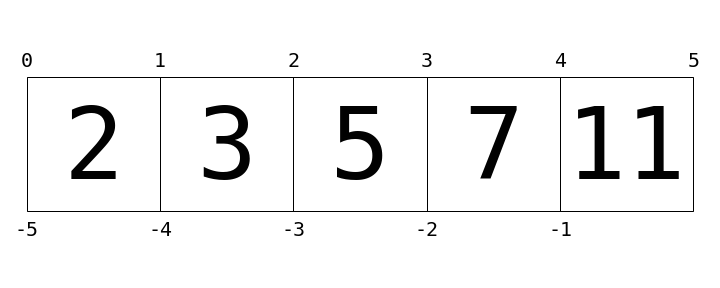
\includegraphics[width = .55\textwidth]{list_indexing.png}
\caption{Indexing (\link{https://jakevdp.github.io/WhirlwindTourOfPython/06-built-in-data-structures.html}{From \cite{vanderplas2016whirlwind}}).}
\label{fig:while}
\end{center}
\end{figure}


%% Slicing

\bigskip

\noindent While indexing pulled out a single element, we can also \emph{slice} to pull out a sublist. 


\begin{lstlisting}[language = Python]
# Get specific items
['Jack', 'Jill', 'and', 'hill', 'over', 'ran', 'the']
print(fine_list[0:2])
print(fine_list[-2:]) \end{lstlisting}

\noindent The first print statement will print elements 0 and 1 in a list. The last print statement will print a list of just the last two elements. Why is slicing done this way? Why does the numbering start at zero and why is the upper bound excluded? It's more of a computer science convention than a Python-specific one. \cite{ramalho2015fluent} (freely downloadable from Columbia Library) addresses this on page 33 and Dijkstra provides some reasoning \link{https://www.cs.utexas.edu/users/EWD/transcriptions/EWD08xx/EWD831.html}{here}. Those reasons are basically:
\begin{enumerate}
    \item The length of the list is more obvious. \code{fine_list[0:2]} contains 2-0=2 elements. And \code{fine_list[:4]} contains four elements. 
    \item It's easy to partition a list. \code{fine_list[:3]} and \code{fine_list[3:]} don't overlap. 
\end{enumerate}



%% Mutability 
\bigskip

\index{mutability}
\noindent Lists are \emph{mutable}, meaning that we can change their contents.

\begin{lstlisting}
# Friend drama
my_best_friends = ['Richard', 'Spiro']
print(my_best_friends)
my_best_friends[1] = 'Gerald'
print(my_best_friends)
\end{lstlisting}


Mutability has consequences when you are assigning one variable to be equal another. By changing \code{b}, which is made from \code{a}, we also change \code{a}. 

\begin{lstlisting}
a = [1,3,5]

b = a
b[2] = 99

print(a)
print(b)
\end{lstlisting}

This was \emph{not} the case for immutable objects like integers, floats, and strings. 

\begin{lstlisting}
a = 1
b = a
a += 1

# b and a are not the same
print(a)
print(b)
\end{lstlisting}



However, we don't see the same effect on mutable objects when reassigning them. 

\begin{lstlisting}
a = [1,3,5]

b = a
b = b[0:1]

# b and a are no longer pointing to the same list
print(a)
print(b)
\end{lstlisting}

Just when ``mutating'' them. 

\begin{lstlisting}
a = [1,3,5]

b = a
b = b.append(7)

# b and a are pointing to the same list
print(a)
print(b)


# This also does the same
a = [1]
b = a

a += [1]

# b and a are pointing to the same list
print(a)
print(b)
\end{lstlisting}

\chapter{Repetition Structures}
%\scalebox{0.8}{\textit{Reference: Gaddis Chapter 4}}

Repetition structures (loops) are one of the best justifications for moving from Excel to Python (though they are not unique to Python). A ``program''
in Excel is a serious of keystrokes and clicks. You might create a report for your company that is specific to one
market and you'll need to replicate the same report for a different market. Perhaps you could write a macro, but
I think you'll find working in Python to be easier. In Python, we can do this in a loop. We can have a program that makes the report and we
can iterate through the different markets to apply the program to each and create the specific reports (using a for loop).

We also introduce the idea of an \emph{iterable} object. 


\section{While Loops}
 
The \textbf{while loop} is a condition-controlled loop. Figure \ref{fig:while} illustrates the logic well.

%% Figure
\begin{figure}[h!] 
\begin{center} 
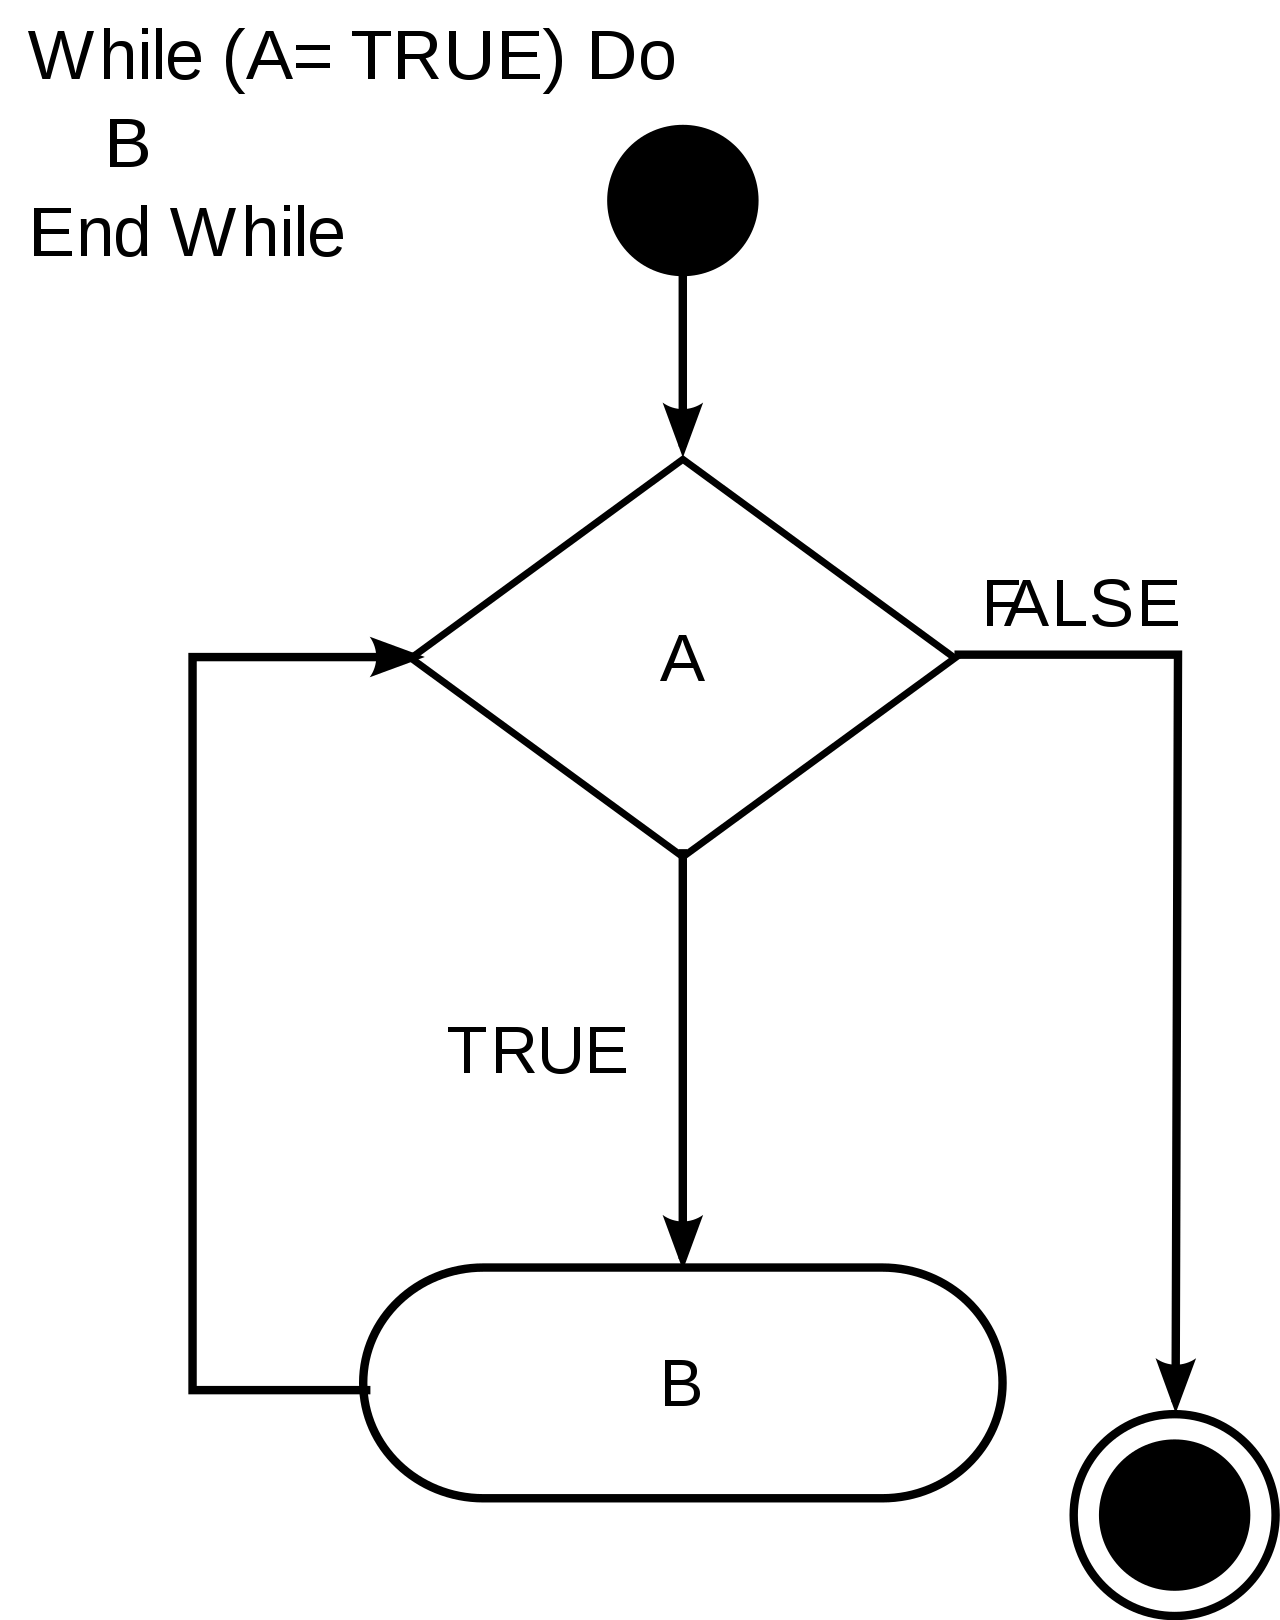
\includegraphics[width = .55\textwidth]{while_loop.png}
\caption{While loop logic (\textcolor{blue}{\href{https://en.wikipedia.org/wiki/While\_loop}{Wikipedia}}).}
\label{fig:while}
\end{center}
\end{figure}


\smallskip

\noindent The statement inside a while loop executes as long as the condition evaluates to True.

\begin{lstlisting}[language = Python]
# Rest on the seventh day
day_of_week = 1
while day_of_week < 7:
    print('work')
    day_of_week += 1 \end{lstlisting}


\smallskip
\noindent Beware the infinite loop. Be confident that your test condition will have a way of becoming False, otherwise
you might notice that your program never finishes. 

\smallskip

\noindent Let's consider an infinite series, $\sum_{i=0}^\infty 2^{-i} =  1 + \frac{1}{2} + \frac{1}{4} + \frac{1}{8} + \dots = 2$.
We could try to calculate this with a while loop if we didn't know the sum converged to two.

\begin{lstlisting}[language = Python]
# Sum of a geometric series
the_sum = 0
idx = 0
increment = 2 ** -idx

while increment > 0:
    # Increase the sum by the current increment
    the_sum += increment
    
    # Advance the index in the sum and calculate a new increment
    idx += 1
    increment = 2 ** (-idx) \end{lstlisting}
    
\smallskip

\noindent Does this loop make you nervous? In fact, the loop will terminate because we will eventually hit machine zero.
I found the loop to terminate at the increment $2^{-1075}$ and the resulting sum to be two. But it should make you nervous.
You might instead decide on some level of precision and use a test condition like 
\lstinline[language=Python]{increment > .0005}, in which case you could find a bound on the error with some math.
Doing that math is not part of this course, (un)fortunately.


\section{For Loops} 
\label{sec:forloop}

For loops execute the attached code based on some iteration. The code might depend on a variable that is actually changing
with the iteration. 

\begin{lstlisting}
#Dr. Seuss
for item in [1,2,'red','blue']:
    print(item, 'fish')  
\end{lstlisting}

The general structure is 
% random Pascal language to avoid highlighting
\begin{lstlisting}[language = Pascal] 
for <iteration_variable> in <iterable>:
    <program>
\end{lstlisting}
The iteration variable should be chosen to maximize readability. 

Sometimes you find definitions for \textbf{iterable} that are circular, like ``objects that can be iterated over.'' It's something where we can traverse through distinct values. So far, the iterables we have seen are strings and lists. A for loop will iterate over a list one element at a time, according to the ordering in the list. A for loop iterates over a string one character at a time. There are several more types of iterable objects, but for now the only additional one we'll introduce is that created by \code{range(start, stop, step)}, which allows you to iterate over integers from \code{start} (inclusive) to \code{stop} (exclusive) according to the \code{step} parameter. By default, \code{start = 0} and \code{step = 1} so these are optional arguments. You can check what is included in a particular call to \code{range()} by examining \code{list(range(start, stop, step))}.

\smallskip

\noindent The for clause tells Python to execute the statement once for every item in the iterable, which is
in this case the object \code{[1,2,'red','blue']}. This is a \emph{list}, a kind of 
compound data object that can store other objects in sequence by separating them with commas and putting
them inside square brackets. Below we use \code{range(5)} instead of a list, which you
can think of as generating an iterable object of integers from 0 to 4 (5 is not included, but the length is 5).


\smallskip

\noindent Or you might just want to execute a specific set of statements some number of times.


\begin{lstlisting}[language = Python]
# Tubthumping by Chumbawamba
for item in range(5):
    print("I get knocked down, but I get up again.")
    print("You are never gonna keep me down.") \end{lstlisting}

\smallskip

\noindent For both of the examples above, \lstinline[language = Python]{item} is the \emph{variable}. However, notice
the print statement only depends on the variable in the first example.

\smallskip
\noindent You can even iterate over the characters in a string.

\begin{lstlisting}[language = Python]
# Cheer
word = 'PYTHON'
for char in word:
    print("Give me a",char, '!')
    print("    ", char)
print("What's that spell?")
print("    ",word) \end{lstlisting}


\subsection{Nested Loops}

A loop that is inside another is called \emph{nested}.

\smallskip
\noindent Think about how Python executes code line by line. What order of output do you expect from this program?


\begin{lstlisting}[language = Python]
# Nested Loop
for x in ['wee', 'bee']:
    for y in ['bop', 'dop']:
        print(x,y) \end{lstlisting}

If it helps, the above is a simplification of the following. 


\begin{lstlisting}
# Nested Loop
x = 'wee'
for y in ['bop', 'dop']:
    print(x,y) 

x = 'bee'
for y in ['bop', 'dop']:
    print(x,y)   
\end{lstlisting}



\smallskip


\chapter{Functions}
\noindent \scalebox{0.8}{\textit{Reference: \cite{lubanovic2019introducing} Chapter 9}}

\emph{Functions} make your code easier to read and write by performing a certain task based on some number of arguments the function takes. Whenever you find yourself copying and pasting code in a program, you should ask yourself if you shouldn't be using a function instead. 

% unplaced: you can put functions in lists but not operators 

\section{Detour: Callables and Functions}

It's a common mistake to call more things functions than actually are functions. There are other things like methods and classes you'll be formally introduced to later and that have a similar feel. Classes and functions are both \emph{callables}, just meaning something you can call by using parentheses and sometimes arguments inside those parentheses.

Consider the code and output below (pasted from the Terminal in VSCode). 
\begin{lstlisting}[language = Python, keywordstyle = \color{black}, stringstyle = \color{black}]
>>> list
<class 'list'>
>>> len
<built-in function len>
>>> callable(len)
True
>>> callable(list)
True
>>> callable
<built-in function callable>
>>> callable(callable)
True
\end{lstlisting}


\section{Function Basics}

In math, you might define a function $f(x) = x^2$. Just as $f$ does something with $x$, a function like 
\code{print} does something with whatever input we pass inside the parentheses. However, an argument/parameter is not always necessary or even allowed depending on the function. In the example below, we define our first function.

\begin{lstlisting}
def your_annoying_friend():
    print("crypto")
\end{lstlisting}

A function definition is begun with the keyword \code{def}. Then you give the function name and input arguments inside parentheses. After the parentheses there is a colon. Then the code dictating what the function does is indented below.


Our function \code{your_annoying_friend} takes no arguments. No matter how many times you call \code{your_annoying_friend}, all it does is print \code{'crypto'}. Try passing an argument inside, like \code{your_annoying_friend('new conversation topic')}, but you'll only get an error because the function is not defined to accept arguments. Further this function actually \emph{returns} nothing because there is no \emph{return statement}. Try running \code{a = your_annoying_friend()}. The variable \code{a} has the value \code{None}, the NoneType (see \cite{lubanovic2019introducing} page 144 for a brief discussion). 


We'll introduce return statements shortly, but first, let's include an argument in a new function. Consider the cheer we made in Section \ref{sec:forloop}. We can make this into a function so that it works for any value of \code{word}.

\begin{lstlisting}
# Cheer
word = 'PYTHON'
for char in word:
    print("Give me a",char, '!')
    print("    ", char)
print("What's that spell?")
print("    ",word) \end{lstlisting}

\begin{lstlisting}
# Cheer Function
def cheer(word):
    ''' Doc string '''
    for char in word:
        print("Give me a",char, '!')
        print("    ", char)
    print("What's that spell?")
    print("    ",word) \end{lstlisting}
    
    
 A function will return a value once it reaches a return statement, begun with the keyword \code{return}. Once the return statement is reached, the function quits executing and any leftover bits of the program are abandoned. Call the function \code{one} below. You'll find that \code{"testing"} is never printed because it comes after \code{return 1}. We can say this function accepts no parameters and always does two things: \emph{prints} \code{"Coming right up."} and \emph{returns} \code{1}.
 
\begin{lstlisting}
def one():
    print("Coming right up.")
    return 1
    print("testing")
\end{lstlisting}


\subsection{Naming}

The same rules for naming variables apply to naming functions. Again, see \link{https://www.python.org/dev/peps/pep-0008/}{PEP 8}. Readability counts. 

 
\section{Arguments and Parameters}
 
I might slip, but there is technically a difference between \emph{arguments} and \emph{parameters}. \cite{lubanovic2019introducing} tells us the values you pass into the function are the arguments. Those values are copied the corresponding \code{parameters} inside the function. In the below, \code{add} is defined and called with arguments \code{1} and \code{2}, and these are copied to the parameters \code{x} and \code{y}.

\begin{lstlisting}
def add(x,y):
    return x + y
    
add(1,2)
\end{lstlisting}
 
 
 The order of your arguments matters. 
 
 \begin{lstlisting}
 def investment_strategy(buy, sell):
    print("buy", buy)
    print("sell", sell)
 \end{lstlisting}
 
 Calling \code{investment_strategy('high', 'low')} and \code{investment_strategy('low', 'high')} produce very different ideas. These arguments are \emph{positional arguments}, in that they are copied to their parameters based on the ordering. If that produces confusion, you can instead use \emph{keyword arguments}. 
 
 \begin{lstlisting}
 investment_strategy(sell = 'high', buy = 'low')
 \end{lstlisting}
 
 You can also specify \emph{default} parameter values so that you don't have to pass an argument. This is demonstrated in the definition below.
 
\begin{lstlisting}
def my_favorite_class(a = 'Python'):
    print(a, "!", sep = '')
\end{lstlisting}
 
 
\subsection{A mutability gotcha}

The default arguments are evaluated once when a function is defined.\footnote{See \link{https://docs.python-guide.org/writing/gotchas/}{common gotchas} from \cite{reitz2016hitchhiker} and \cite{lubanovic2019introducing} page 147.} This can create something unexpected when using a mutable default argument---if you mutate the argument, it will stay mutated for future use of the function. 


\begin{lstlisting}
def risky_function(x, l = []):
    l.append(x)
    return l
\end{lstlisting}

Run \code{risky_function('a')} twice. You might expect \code{['a']} to be returned in both instances, but you will get \code{['a','a']} on the second call. You can avoid this behavior with something like the following. 

\begin{lstlisting}
def workaround(x, l = None):
    if l == None:
        l = list()
    l.append(x)
    return l
\end{lstlisting}

\section{Annotation and Documentation}

A function can include a documentation string (docstring) and annotation regarding the intended argument data types. Annotations for a parameter are to be preceded with a colon. An annotation for the output can be created with \code{->} before the annotation, between the closed parenthesis and colon. Python simply stores this information. There are no checks or enforcement. Below, the default argument for \code{y} doesn't even obey the annotation. 

\begin{lstlisting}
def annotated_function(x:str, y:'int > 0' = -1) -> bool:
    "Sample Docstring"
    return x
    
# Violates the annotation but still runs
annotated_function(1, -99)
\end{lstlisting}

\index{assert}
If you want checks enforced, you will have to code them in yourself. One way to do that is by using an assert statement inside your function. With \code{assert} and then a boolean expression, your code will break if the expression is false.

\begin{lstlisting}
def assertive_function(x: int):
    assert type(x) == int
    return x
\end{lstlisting}

This doesn't help the user of your code very much. So instead, you might want to create an exception of your own to explain what went wrong. This is done with \code{raise}, which will be covered in more detail in Chapter \ref{chapter:except}.\footnote{\link{https://docs.python.org/3/tutorial/errors.html\#raising-exceptions}See also the {official documentation} for raising exceptions.}

\begin{lstlisting}
def integer_identity(x: int):
    if type(x) != int:
        raise TypeError("x must be an integer")
    return x
\end{lstlisting}


You can access function definitions and documentation using \code{?function_name} or \code{help(function_name)}.



\section{Local and Global Variables and Namespaces}

As we keep creating keyword parameters in our functions, or additional variables inside the function, you might start to wonder what if I had already used that keyword as a variable name? The below shows that no conflict arises. \code{foo} will not overwrite the variables \code{a} and \code{b}, and \code{foo} still operates without interference from those variables being previously defined. 
 
\begin{lstlisting}
a = 10
b = 10
def foo(a = 1):
    b = 2*a
    return b

x = foo(a = 0)
print(x)
print(a, b)
\end{lstlisting}

The reason this all behaves so well is that there is a global \emph{namespace} in which \code{a} and \code{b} are defined as \code{10}. And there is a separate namespace for the function \code{foo}, where \code{a} and \code{b} can exist independently, just as ``die'' can mean one thing in England and another thing in Germany. 

\begin{center}
    \link{https://www.youtube.com/watch?v=gaXigSu72A4}{
\includegraphics[width = .56\textwidth]{images/diebartdie.jpeg}}
    
Above: an argument over namespaces from \link{https://www.youtube.com/watch?v=gaXigSu72A4}{\emph{The Simpsons}}.
\end{center}


There are local variables and there are global variables. A variable's \emph{scope} is the part of a program where the variable can be accessed. Variables created inside a function are local and their scope is the function. Different functions can have local variables of the same name without creating any kind of interference thanks to the separate namespaces.
 
%We'll return to this when we cover modules and IPython.\footnote{remind me}
 
\section{Anonymous Functions}

Anonymous functions are created as lambda functions. The main use for this for functions that have a very short definition and that might only be used once in a program, or perhaps as an argument in a higher-order function (covered in Section \ref{sec:higher}).

\begin{lstlisting}
def simple_function(x):
    return 1 * (x > 0)
\end{lstlisting}

The above can be replaced by 
\begin{lstlisting}
simple_function = lambda x: 1 * (x > 0)
\end{lstlisting}

We can even do something a little more complicated. 

\begin{lstlisting}
simple_but_complicated = lambda x, y=-9: 1 * (x > y)
\end{lstlisting}%\footnote{Here we have 1 times a boolean. \code{1*True} is \code{True} and \code{1*False} is \code{False}.}

 
\section{Higher-Order Functions Like \texttt{map}}\label{sec:higher}
 
A function that takes another function as an argument is a higher-order function (see \cite{ramalho2015fluent}). Two examples are the built-in functions \code{sorted} and \code{map}.

\index{sorting}
\code{sorted} takes an iterable and returns a new sorted iterable as long as every element of the iterable can be compared. Observe \code{sorted([3,1,2]) == [1, 2, 3]}. What makes \code{sorted} a higher-order function is the optional \code{key} argument. 

\index{map}
\code{map} takes a function and applies it to every element in the iterable. It returns something call an iterator, holding the results. You can convert the iterator to a list using \code{list()} to see the results. 

\begin{lstlisting}
# Square the elements of a list
# [0,1,4,9]**2 doesn't work

f = lambda x: x**2
print(map(f, [0,1,2,3]))
print(list(map(f, [0,1,2,3])))
\end{lstlisting}

\section{Examples}

\begin{lstlisting}
def letter_value(letter):
    
    # convert to lowercase
    letter = letter.lower() 
    # according to some blog
    if letter in 'eaionrtlsu':
        return 1
    elif letter in 'dg':
        return 2
    elif letter in 'bcmp':
        return 3
    elif letter in 'fhvwy':
        return 4
    elif letter == 'k':
        return 5
    elif letter in 'jx':
        return 8
    elif letter in 'qz':
        return 10
    else:
        return "not a valid letter"
    
def word_value(word):
    return sum(map(letter_value, word))
\end{lstlisting}

Now run \code{sorted(['friends', 'enemies', 'burgers', 'I', 'a', 'I', 'I'], key = word_value)}.

 
 
 \subsection{Exercise!}
 \begin{lstlisting}
# Find a nearby multiple of five
def find_close_multiple_of_five(num):
    # check if multiple of five
    is_multiple = num % 5 == 0
    while is_multiple not True:
        num += 1
        is_multiple = num % 5
    return num \end{lstlisting}
    
    


\chapter{Exceptions}\label{chapter:except}


The \link{https://www.python.org/dev/peps/pep-0020/}{Zen of Python} advises us that ``Errors should never pass silently.'' 


\section{Exceptions}
\scalebox{0.8}{\textit{Reference: \cite{lubanovic2019introducing} Chapter 9}}
\medskip

Occasionally, you might ask Python to do something impossible. Try running \code{1/0}. You will get an error message, \code{ZeroDivisionError}. Robust code should deal with this possibility intelligently. This is especially true when writing functions. You can avoid errors by writing your code to prevent them from occurring. Or, you might write code that responds to errors. For more on the built-in exceptions, follow \link{https://docs.python.org/3/library/exceptions.html}{this link}.

\smallskip
\noindent Here's an example of avoiding the division by zero error. 

\begin{lstlisting}[language = Python]
def pct_change(old, new):
    delta = new - old
    if old != 0:
        pct = 100 * delta / old
        return pct
    else:
        return "Not defined."\end{lstlisting}
        
\smallskip
\noindent Here's an example of dealing with the error, which requires \code{try} and \code{except} statements.

\begin{lstlisting}[language = Python]
def pct_change1(old, new):
    delta = new - old
    try:
        pct = 100 * delta / old
        return pct
    except ZeroDivisionError:
        return "Not defined."\end{lstlisting}
        
\smallskip
\begin{lstlisting}[language = Python]
# Will this work?
def pct_change2(old, new):
    delta = new - old
    try:
        pct = 100 * delta / old
        return pct
    return "Not defined."\end{lstlisting}
    
    
\smallskip
\noindent A \code{try} must be paired with an \code{except}, so the definition of \code{pct_change2} will not work. There must be an \code{except} and, as we use in \code{pct_change1}, it's a good idea to use the form \code{except ExceptionName}. This tells Python what code to run when a certain exception is encountered.


\smallskip
\begin{lstlisting}[language = Python]
def pct_change3(old, new):
    try:
        delta = new - old
    except TypeError:
        return "Use ints or floats."
    try:
        pct = 100 * delta / old
        return pct
    except ZeroDivisionError:
        return "Not defined."\end{lstlisting}



\smallskip

\noindent The following function, \code{pct_change4}, actually won't run properly if you attempt to execute \code{pct_change4(1,'cheese')}. Can you figure out why? Think about the ordering of the code. 

\begin{lstlisting}[language = Python]
def pct_change4(old, new):
    delta = new - old
    try:
        pct = 100 * delta / old
        return pct
    except ZeroDivisionError:
        return "Not defined."
    except TypeError:
        return "Use ints or floats."\end{lstlisting}
        
\smallskip
\noindent You do not need to specify the error type in your \code{except} statement. Sometimes this might hide errors that you do want to be surfaced or stop the execution of a program, so use these blanket exceptions carefully. 

\begin{lstlisting}[language = Python]
def pct_change5(old, new):
    try:
        delta = new - old
        pct = 100 * delta / old
    except:
        return "An error occurred."
    return pct\end{lstlisting}
    
\smallskip
\noindent You might use a blanket except after handling specific errors. 

\begin{lstlisting}[language = Python]
def pct_change6(old, new):
    try:
        delta = new - old
        pct = 100 * delta / old
        return pct
    except ZeroDivisionError:
        return "You can't divide by zero."
    except:
        return "An error occurred."\end{lstlisting}
        
\smallskip
\noindent It can be useful information to know what type of exception your code generates. In that case, you can access and print that error. 

\begin{lstlisting}
try:
    'a' + 1
except Exception as e:
    print(e)\end{lstlisting}
    
\smallskip
\noindent The use of \code{Exception} above matters. Compare these two programs.

\begin{lstlisting}[language = Python]
try:
    'a' + 1
except TypeError as e:
    print(e)\end{lstlisting}
    
\begin{lstlisting}[language = Python]
try:
    'a' + 1
except ValueError as e:
    print(e)\end{lstlisting}
    
\smallskip
\noindent Only the first program above actually handles the exception. 


\smallskip
\noindent Now, we consider the use of \code{else} and \code{finally} statements after a \code{try}/\code{except}. An \code{else} clause can be added after the \code{except} clauses, and the statements in the \code{else} clause are executed only if no exceptions were raised. The \emph{else} is then in contrast to the raising of exceptions, in a similar style as when an \code{else} might be used in complement to an \code{if}. What output do you expect from the following program? What if we changed the value of \code{denom}?

\begin{lstlisting}[language = Python]
denom = 0
try:
    print(2 / denom)
except Exception as e:
    print(e)
else:
    print(3 / denom) \end{lstlisting}

\smallskip
\noindent Here are slightly more complicated examples. Try running them to see what happens.

\begin{lstlisting}[language = Python]
products = ['bike','treadmill']
try:
    print(products[2])
except IndexError as e:
    print(e)
except Exception as e:
    print(e, 'other error')
else:
    print(products[2], '!') \end{lstlisting}
    
\begin{lstlisting}[language = Python]
products = ['bike','treadmill']
try:
    print(products[1])
except IndexError as e:
    print(e)
except Exception as e:
    print(e, 'other error')
else:
    print("Else block time")
    print(products[2], '!') \end{lstlisting}
    
    
\smallskip
\noindent Next, we introduce the \code{finally} clause. Whereas the \code{else} block was executed when no exceptions were raised, the \code{finally} closed is executed no matter what. This \link{https://stackoverflow.com/questions/11551996/why-do-we-need-the-finally-clause-in-python}{StackExchange post} helps explain the unique usefulness of this, but we won't got into that much detail.

\begin{lstlisting}[language = Python]
products = ['bike','treadmill']
idx = 2
try:
    print(products[idx])
except Exception as e:
    print(e, 'other error')
finally:
    print('End') \end{lstlisting}


\chapter{More Data Structures}
\section{Tuples}
\scalebox{0.8}{\textit{Reference: \cite{lubanovic2019introducing} Chapter 7}}

A \emph{tuple} is a lot like a list. Whereas lists used square brackets (\code{[]}), a tuple uses parentheses, (\code{()}). Like lists, we can index and slice a tuple. The main difference is that tuples are immutable. We cannot reassign the element at a particular index. 

\begin{lstlisting}[language = Python]
example_list = ['bike','treadmill']
example_tuple = ('bike','treadmill')

example_list[1] = 'treadmill'
example_tuple[1] = 'spacecraft' # This will throw an error\end{lstlisting}

Note we can convert lists and tuples, similar to the way we could convert floats and strings (\code{int("1"), str(1)}).

\begin{lstlisting}[language = Python]
example_list = ['bike','treadmill']
example_tuple = ('bike','treadmill')

print(list(example_tuple))
print(tuple(example_list)) \end{lstlisting}


It might be hard to see immutability as an advantage, but this does make tuples to be safer objects. You won't accidentally screw them up (unless at the very beginning). There is another more definite advantage to tuples. They are processed faster. Processing speed will not be a practical concern in this class, but it could be a concern in your professional career. 


\subsection{Tuple Assignment}

Tuples can also be created without parentheses. 

\begin{lstlisting}
friends = 'Big Bird', 'Snuffleupagus'
\end{lstlisting}

Or you can we can create individual variable names with something like the following. 

\begin{lstlisting}
main, sidekick = 'Mitt', 'Paul'
\end{lstlisting}

\noindent This is kind of nice and or tricky when thinking about reassigning variables. Compare the following.

\begin{lstlisting}
apples = 10
pies_possible = 2

apples, pies_possible = 2*apples, apples/5
print(apples, pies_possible)

apples = 10
pies_possible = 2

apples *= 2
pies_possible = apples/5
print(apples, pies_possible)
\end{lstlisting}

\subsection{Unpacking}

Tuples can be \emph{unpacked} with an asterisk, \code{*}, to create a starred expression. This is useful when the tuple structure isn't wanted, like when you don't want nested tuples. 

For example, let's start with a tuple, \code{friends = 'Antonin', 'Ruth'}. We might want to add these to a larger tuple. Let's try: 

\begin{lstlisting}
former_justices = 'Breyer', friends
\end{lstlisting}

This results in a nested tuple \code{('Breyer', ('Antonin', 'Ruth'))}. We should unpack \code{friends}.

\begin{lstlisting}
former_justices = 'Breyer', *friends
\end{lstlisting}

Now we have a flat tuple \code{('Breyer', 'Antonin', 'Ruth')}. This would also work if friends where a list. That is, we get the same value for \code{former_justices} if we instead ran \code{former_justices = 'Breyer', *list(friends)}.

Next, unpacking can be useful in use with functions when you'd like each element of the tuple to be processed as a new positional argument.

\begin{lstlisting}
def heart(a,b):
    return a + " <3 " + b
# heart(friends) returns an error
print( heart(*friends) )
\end{lstlisting}

\subsection{Tuples vs. Lists}

Recall the primary difference between lists and tuples: lists are mutable and tuples are not. It might be hard to see immutability as an advantage, but this does make tuples to be safer objects. You won't accidentally screw them up (unless at the very beginning).

There is one definite advantage to tuples. They are processed faster. Processing speed will not be a practical concern in this class, but it could be a concern in your professional career. 
\section{The \code{in} Operator}

The \code{in} operator allows you to determine if an element is contained in a list or tuple. In Python, the statement \code{x in A}, where \code{A} is a list, mirrors the mathematical statement $x\in A$ where $A$ is a set. While we never formally introduced \code{in}, we've already seen it in for loops with the for clause, \code{for item in range(10):}, for example.

\smallskip

Realize that for numerics, \code{in} will evaluate to true as long as the element is equal (\code{==}) to something in the list. That means a float can be \code{in} a list of integers.

\begin{lstlisting}
chapters_on_midterm = [2,3,4,4,5,6,7,8,9]

# confirm all integers
for item in chapters_on_midterm:
    print(item, type(item))

# This is certainly True
bool1 = 2 in chapters_on_midterm

# What about this? 
bool2 = 2.0 in chapters_on_midterm # This is True!
\end{lstlisting}

\smallskip

\noindent Finally, you can use \code{not in} as you might expect. The statement \code{x not in some_list} if there is no element \code{y in some_list} that is equal to \code{x}.

\section{List Methods}
\scalebox{0.8}{\textit{Reference:\cite{lubanovic2019introducing} Chapter 7}}

Python methods are like functions, but they are associated with objects.

\smallskip
\noindent Functions look like this: \code{sorted(some_list)}\\
\noindent Methods look like this: \code{some_list.sort()}

\smallskip
\noindent For now, we can proceed thinking of them just as functions with this syntax. 

\smallskip
The function \code{sorted()} and the method \code{.sort()} do the same thing in some sense---both can be used to sort a list. They are different in that \code{sorted()} returns a new sorted list without mutating \code{some_list}. The method \code{.sort()} doesn't return anything; it mutates the list into a sorted list. This difference isn't a property of functions and methods. The difference is particular to \code{sorted()} and \code{.sort()}. 

\begin{lstlisting}
# Demonstration of sorted() and .sort()

presorted_list = [1,2,3,4]
alt_list = [1,4,2,3]

c1 = alt_list == presorted_list
print(c1)

c2 = sorted(alt_list) == presorted_list
print(c2)

c3 = alt_list == presorted_list
print(c3)

alt_list.sort()

c4 = alt_list == presorted_list
print(c4)
\end{lstlisting}


\smallskip

Other important list methods include \code{.append()} and \code{.index()}. \code{.append()} requires an argument---an element to be added to the end of the list.

Running \code{some_list.append(x)} does the same thing \code{some_list += [x]} would accomplish.

\begin{lstlisting}
# .append() Demonstration
ones = list()

ones.append(1)

print(ones)

ones += [1.0] # Recall this is the same as ones = ones + [1.0]

print(ones)
\end{lstlisting}


\smallskip

\noindent Next, the \code{.index()} method helps us find the index of the first instance of a particular element in a list. This method requires an argument, and \code{some_list.index(x)} returns the minimum index of \code{x} in \code{some_list}. 


\begin{lstlisting}
# .index() Demonstration
ones = [1, 1.0] 

print(ones.index(1))

print(ones.index(1.0)) 

# There is no distinction between int and float
print(ones.index(1.0) == ones.index(1)) 
\end{lstlisting}

\smallskip
\noindent \textbf{Exercise:} Remove the duplicates from a list.

\begin{lstlisting}
big_list = [1,2,4,2,12,4,12,234,1,1,1,1] # a lot duplicates

big_list_without_dups = []

for element in big_list:

  if element not in big_list_without_dups:
 
    big_list_without_dups.append(element) 
    
    
## Alternate version

big_list_without_dups_alt = []

idx = 0 # keep track of index of each element
for element in big_list:
    # Add the element if it's the first time we've seen it in big_list
    first_index = big_list.index(element)
    if idx == first_index:
        big_list_without_dups_alt.append(element)
        
    # Advance the index for the next element
    idx += 1
\end{lstlisting}


\section{Strings}
\scalebox{0.8}{\textit{Reference: \cite{lubanovic2019introducing} Chapter 5}}

Strings behave like lists in terms of indexing, slicing, and iterating. Strings are immutable however.

The \code{in} operator can be used on strings to test if one string is a substring within another string. 

\begin{lstlisting}[language = Python]
for char in 'team':
    print(char, char in team):
    
print("I" in 'team')
\end{lstlisting}


Important string methods include \code{.upper()}, \code{.lower()}, \code{.isalpha()}, \code{.split()}, and \code{.replace()}. 

The \code{.upper()} and \code{.lower()} methods return a new string in uppercase or lowercase letters, respectively. These do not mutate the original string and no arguments are necessary. 

The \code{.isalpha()} method returns a boolean, stating whether or not the string contains all alphabetical characters (this is different than not being a integer data type for example---a string might still contain a numeric character). 

\begin{lstlisting}
# In case you can't trust your eyes for l vs 1. 

lowercase_L = "l"
one = "1"

for item in lowercase_L, one:
    print(item, item.isalpha())
\end{lstlisting}

The \code{.replace()} method takes two arguments. It returns a new string that replaces every instance of the first argument with the second argument. The function below returns a more muted string by eliminating all capital letters and converting exclamation marks to periods. 

\begin{lstlisting}
def lower_your_voice(string):
    lowercase = string.lower()
    not_exclamatory = lowercase.replace("!", ".")
    return not_exclamatory
    
print(lower_your_voice("Your card was declined!"))
\end{lstlisting}

\smallskip
The \code{.split()} method requires an argument and returns a list, dividing a string into substrings based on the argument. This is especially useful for splitting a sentence into its individual words.

\begin{lstlisting}
invisible_hand = "It is not from the benevolence of the butcher that we expect our dinner but from their regard to their own interest"

the_words = invisible_hand.split(" ")

print(the_words)

# Note what happens when you split on the first or last character in a string

laugh = 'hahahahah'

split_laugh = laugh.split('h')

print(split_laugh)

# Note what happens when you pass no argument
print(laugh.split())

# This gives an error. You can't split on a zero-length separator.
laugh.split("")
\end{lstlisting}



\section{Dictionaries}
\scalebox{0.8}{\textit{Reference: \cite{lubanovic2019introducing} Chapter 8}}
\smallskip

Dictionaries allow us to store key-value pairs. It's kind of like having one row in a table. Keys are like column names and values are the row-column cell value. Key-value pairs are created as \code{key: value}, then separated by commas and wrapped in curly braces, \code{\{\}}, to create a dictionary. Consider the example below.

\begin{lstlisting}
workout = {'user': 'Velma', 'fitness_discipline': 'cycling', 'instructor': 'Matt Wilpers'}
\end{lstlisting}

A specific value is access by indexing the dictionary by the key. 

\begin{lstlisting}
print(workout['user'])
\end{lstlisting}

\smallskip
We can add new key-value pairs by assigning the value to the dictionary at that key. 

\begin{lstlisting}
# Build a dictionary from scratch
journal = dict() # creates an empty dictionary, can also use {}

journal['2020-10-03'] = "Today I learned a lot of Python. It was buckets of fun."
\end{lstlisting}

\smallskip
\noindent The \code{in} operator works on dictionaries by searching the keys. 

\begin{lstlisting}
# Help translate bad journalism
media_translator = {'is caused by': 'is correlated with'}

print('is caused by' in media_translator)
print('is correlated with' in media_translator)
\end{lstlisting}


You can access the keys with the \code{.keys()} operator and values with the \code{.values()} operator. So \code{x in some_dict} is actually a shorthand for \code{x in some_dict.keys()}.

\smallskip

\noindent Dictionary keys must be immutable. Tuples are fine. Lists are not. 

\begin{lstlisting}
# Economist Santa

gifts = {} # could also use dict() here 

for child in ['Anna', 'Boris']:
    for year in [2020, 2021]:
        
        key = child, year # this is a tuple just like (child, year)
        
        gifts[key] = 'money'
        
print(gifts)
\end{lstlisting}




\section{Sets}
\scalebox{0.8}{\textit{Reference: \cite{lubanovic2019introducing} Chapter 8}}
\smallskip

I find sets to be underrated. They give flexibility in analysis because they allow for quick intersections and unions (e.g. find and analyze users who did this \emph{and/or} that).

\smallskip
\noindent Sets are unordered and duplicates are ignored. We construct them like lists, but use \code{\{\}} instead of \code{[]}. Note that to create an empty set, you should use \code{set()} because \code{\{\}} creates an empty dictionary. 


\smallskip
\noindent Being unordered means it is true that \code{\{1,2\} == \{2,1\}}.


\smallskip
\noindent It's not exactly right to say that sets \emph{can't} have duplicates. You can create a set with duplicate elements and no error will be thrown. But those duplicates are ignored so that the created set object will not in fact have any duplicates. Thus, it is true that \code{\{1,2\} == \{2,1,1,2\}}.


\bigskip Three important methods are \code{.union()}, \code{.intersection()}, and \code{.difference()}. Each of these acts on a set and requires another set as an argument. Intersection and union work like the set operations $\cap$ and $\cup$. The difference method performs set subtraction, $\setminus$. Recall that set subtraction is not commutative; $A\setminus B \neq B\setminus A$ unless $A = B$. 

\begin{lstlisting}
# Union and Intersection

primes = {2,3,5}
evens = {2,4,6}

even_and_prime = primes.intersection(evens)

even_or_prime = primes.union(evens)

for set_ in even_and_prime, even_or_prime: # note we're iterating over a tuple
    print(set_)
    
# Set Subtraction

contiguous_USA = {'New York', 'Kentucky', 'Wisconsin', 'California'} # among other states

tectonic_seceder = {'California'}


print(contiguous_USA.difference(tectonic_seceder))

# We can also use the - operator
print(contiguous_USA - tectonic_seceder)

## More Subtraction 

cold_places = {'Wisconsin', 'Yukon'}

print(contiguous_USA.difference(cold_places))

# Reverse the arguments
print(cold_places.difference(contiguous_USA))
\end{lstlisting}


\bigskip

Now that we've seen these data types, you are well prepared to work with a lot of data you might find in the wild. See the code from class for an example using a public API. 


\chapter{Modules}
\scalebox{0.8}{\textit{Reference: \cite{lubanovic2019introducing} Chapter 11}}

A \emph{module} is a file that contains Python code. Large programs are more manageable when divided into modules. Many functions in the standard Python library are stored in modules. The \code{math} and \code{random} modules are common examples. These shouldn't require additional installation to use if you've downloaded Anaconda. 

To use a module, you must import the module with an import statement, \code{import math} for example. Then any function in that module can be accessed by using the function name, prefixed by the module name and a dot. To use \code{sqrt} from \code{math}, you must use \code{math.sqrt(81)}. 

You can import just a specific function with syntax like the following: \code{from math import sqrt}. Then \code{sqrt} can be accessed without the \code{math.} prefix. Running \code{from math import *} is called a wildcard import and will import every function in the module. 

Finally, you can \emph{alias} a specific module, library, or function with an \code{as} clause. There are conventional aliases for many modules. Pandas, NumPy, and Datetime are libraries we will cover later. These are typically imported with aliasing as in the below. 

\begin{lstlisting}[language = Python]
import pandas as pd
import numpy as np
import datetime as dt
from math import sin as sine # Not a typical alias, but for demonstration
\end{lstlisting}

\subsection{Storing Functions in Modules}
You can create your own module by placing code into a .py file. If that file is in your directory, you can access it with an import statement. In the lecture folder, I've placed a file \texttt{next\_power.py}. Download that and place it in your working directory to try importing it. In Google Colab, you can upload files in the left menu. 

Try the following.

\begin{lstlisting}[language = Python]
import next_power
val = next_power.next_power_of_five(126)
print(val)
\end{lstlisting}

\begin{lstlisting}[language = Python]
import next_power as npow
val = npow.next_power_of_five(44)
print(val)
\end{lstlisting}

\begin{lstlisting}[language = Python]
from next_power import next_power_of_five
val = npow.next_power_of_five(309)
print(val)
\end{lstlisting}

\noindent It's difficult to overstate how helpful this is in creating cleaner and more readable Jupyter notebooks. 


\subsection{Using the \texttt{random} module and \texttt{matplotlib}}

Let's get our hands dirty a bit. 

\begin{lstlisting}[language = Python]
import random
random.seed(33) # pick a seed for reproducibility

number = random.randint(0,1)
\end{lstlisting}


\begin{lstlisting}[language = Python]
# Gambler's Ruin

purse = 100 # starting money

# Keep gambling if you have money
total_gambles = 0
purse_values = [purse]
while purse > 0:
    outcome = random.choice([-1,1]) # win or lose 1 with eve odds
    purse += outcome 
    
    purse_values.append(purse) 
    total_gambles += 1 
\end{lstlisting}

\noindent We can graph this with \code{matplotlib}.

\begin{lstlisting}[language = Python]
import matplotlib.pyplot as plt
plt.plot(range(total_gambles+1), purse_values)
plt.show()
\end{lstlisting}

\begin{center}
    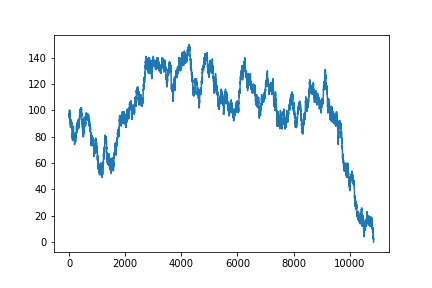
\includegraphics[width = .5\textwidth]{gamblers_ruin.png}
\end{center}

\chapter{Object Oriented Programming}
\section{Object Oriented Programming}
\scalebox{0.8}{\textit{Reference: \cite{lubanovic2019introducing} Chapter 10}}\medskip

So far, our programming has been \emph{procedural}. A program was made of procedures and data might be passed from one procedure to the next. This creates a separation of data and the procedures/operations. As a program grows, this can become more unwieldy. We'll talk about defining classes. While you might get quite far without having to define your own classes, the vocabulary here is important for anyone who wants to be fluent in Python and understand popular libraries like Pandas. 

\smallskip
\noindent \emph{Object-oriented programming} (OOP) centers on creating objects instead of procedures. An object contains both data and procedures. An object's data are its \emph{data attributes}. An object's procedures are its \emph{methods}, which operate on the data attributes. Attributes are like variables and methods are like functions. Bundling data with the code operating on it is called \emph{encapsulation}. 
\smallskip 

\subsection{Classes}

A \emph{class} is code that specifies the data attributes and methods for a particular type of object. A class is like a blueprint and the object is the particular realization. When we previously talked about data types, we were really referencing classes. Run \code{print(type('Hello, World!'))}. Your output should be \lstinline{<class 'str'>}.

\smallskip
\noindent
Classes are defined in the following way. Note, per \link{https://www.python.org/dev/peps/pep-0008/\#class-names}{PEP 8}, class names should follow the CapWords convention. 

\begin{lstlisting}[language = Python]
import random 

class Coin: 

    def __init__(self):
        self.sideup = "Heads"
        self.coin = "Quarter"
\end{lstlisting}

\smallskip
\noindent Run \code{coin = Coin()} and print \code{coin.sideup} and \code{coin.coin}.

So a minimal class definition includes the \code{__init__} \emph{initializer method}. This initializes the objects data attributes. We could instead make these attributes arguments.


\begin{lstlisting}[language = Python]
import random 

class Coin: 

    def __init__(self, sideup = 'Heads', coin = 'Quarter'):
        self.sideup = sideup
        self.coin = coin
\end{lstlisting}

\smallskip
\noindent Take care to note the last two lines in the block above are necessary to create the \code{sideup} and \code{coin} attributes. Now, let's add some methods to our class.

\begin{lstlisting}[language = Python]
import random 

# Simulate a coin that can be tossed

class Coin: 

    def __init__(self, sideup = 'Heads', coin = 'Quarter'):
        self.sideup = sideup
        self.coin = coin

    def toss(self):
        toss_outcome = random.choice(['Heads','Tails'])
        self.sideup = toss_outcome # Here we change the attribute instead of returning a value
\end{lstlisting}

See what happens now. 

\begin{lstlisting}[language = Python]
coin = Coin() # start with a coin that is heads up per class default value
for i in range(100):
    
    print(coin.sideup)
    coin.toss() # toss the coin
\end{lstlisting}

\smallskip
\noindent Here we add a value-returning method. 

\begin{lstlisting}[language = Python]
import random 

# Simulate a coin that can be tossed

class Coin: 

    def __init__(self, sideup = 'Heads', coin = 'Quarter'):
        self.sideup = sideup
        self.coin = coin

    def toss(self):
        toss_outcome = random.choice(['Heads','Tails']) # local variable just like before in defining functions
        self.sideup = toss_outcome # Here we change the attribute instead of returning a value
        
    def get_sideup(self):
        return self.sideup
\end{lstlisting}

Next, we might want to use \emph{hidden attributes}. Before we could externally change \code{sideup} attribute. Perhaps you don't want that to be possible in this or in another setting. Then you can make that attribute private by including two underscores with the init.

\begin{lstlisting}[language = Python]
import random 

# Simulate a coin that can be tossed

class Coin: 

    def __init__(self, sideup = 'Heads', coin = 'Quarter'):
        self.__sideup = sideup
        self.coin = coin

    def toss(self):
        toss_outcome = random.choice(['Heads','Tails']) # local variable just like before in defining functions
        self.__sideup = toss_outcome # Here we change the attribute instead of returning a value
        
    def get_sideup(self):
        return self.__sideup # We need two underscores here too!
\end{lstlisting}

Now for \code{coin = Coin()}, you cannot access the \code{sideup} attribute with either \code{coin.sideup} or \code{coin.__sideup}. The \code{get_sideup()} method becomes necessary to access the private attribute. When making a data attribute private, one might create methods for accessing and changing those attributes. These are called accessor and mutator methods. Or you might call them getters and setters, respectively.


\smallskip
\noindent The \code{__str__} method is designed to indicate an object's emph{state} (the attribute values). 

\begin{lstlisting}[language = Python]
import random 

class Coin: 

    def __init__(self, sideup = 'Heads', coin = 'Quarter'):
        self.sideup = sideup
        self.coin = coin
        
    def __str__(self):
        return "The coin is a " + self.coin + ", and it is " + self.sideup + "."
\end{lstlisting}

This method is accessed not directly, but by printing the object. 
\section{Inheritance}


\code{Inheritance} allows a new class to extend an existing class. This helps with code reusability a bit because we can have super and subclasses. 

We might start with a superclass. Here's an example.

\begin{lstlisting}[language = Python]
class Automobile():

    def __init__(self, gas_tank):
        self.gas_tank = gas_tank
        
    def drive(self):
        self.gas_tank -= 1
\end{lstlisting}

Now let's make a subclass.
\begin{lstlisting}[language = Python]
class HybridCar(Automobile):

    def __init__(self, gas_tank, battery):
        Automobile.__init__(self, gas_tank)
        
        # initialize additional battery parameter
        self.battery = 100
\end{lstlisting}

Try defining \code{prius = HybridCar(50,100)} and running \code{prius.drive()}. It should work. Check \code{prius.gas_tank}. This illustrates basic inheritance of classes. 

\subsection{Polymorphism (G\S11.2)}
Now we demonstrate \emph{polymorphism.} A subclass can have the same methods defined as their superclass. The methods override the superclass. 

\begin{lstlisting}[language = Python]
class HybridCar(Automobile):

    def __init__(self, gas_tank, battery):
        Automobile.__init__(self, gas_tank)
        
        # initialize additional battery parameter
        self.battery = battery
        
    def drive(self):
        self.gas_tank -= .5
        self.battery -= 1
\end{lstlisting}

\smallskip
\noindent Python includes a handy \code{isinstance()} function that helps determine if an object is of a certain class or of an instance of a subclass of that class.

\begin{lstlisting}[language = Python]
print(isinstance(prius, Automobile))
print(isinstance(prius, HybridCar))
\end{lstlisting}

\chapter{IPython}
\section{IPython and Jupyter}



\scalebox{0.8}{\textit{Reference: \cite{mckinney2012python} Chapter 2 and \cite{vanderplas2016python} Chapter 1}}


Thus far, we've been using Google Colab, which runs IPython notebooks. Now, we'll use Jupyter. Basically, we're moving off of the cloud.


\subsection{IPython Basics}
The Jupyter notebook is an interactive document for code, text, data visualization, and other output. Python's Jupyter kernel uses the IPython system, so all of the IPython basics we'll cover will apply to Jupyter notebooks. Beyond simply executing Python code, IPython comes with enhanced features that make coding easier. I've highlighted a few here. Read through McKinney \S2.2 or check the IPython sections from Vanderplas's \link{https://jakevdp.github.io/PythonDataScienceHandbook/01.02-shell-keyboard-shortcuts.html}{Python Data Science Handbook}. 

\smallskip

\noindent \textbf{Tab completion} is a feature that allows you to hit tab following some input and then any variables matching the characters will be displayed. 

\smallskip

\noindent \textbf{Introspection} refers to the ability to place a \code{?} before or after a variable and executing the line will display helpful information about the object. For a function, you'll be shown the \emph{docstring}.

\smallskip
\noindent Notebooks are divided into discrete code cells. You can select multiple with shift and select. Then use \texttt{shift-m} to \textbf{merge cells}. Use \texttt{ctrl-c} to interrupt a command. 

\smallskip
\noindent There are also certain \textbf{magic commands} that begin with a \code{\%}. My favorite are \code{\%\%timeit} and \code{\%load}. See McKinney page 29 for a table of magic commands or Vanderplas \link{https://jakevdp.github.io/PythonDataScienceHandbook/01.03-magic-commands.html}{here}. Another useful magic command when working with your own modules is the \link{https://ipython.org/ipython-doc/3/config/extensions/autoreload.html}{autoreload command}. If you are developing in a separate .py file and prototyping in a notebook, this is very handy. 

\begin{lstlisting}
%load_ext autoreload
%autoreload 2
\end{lstlisting}



\smallskip
\noindent You can run \textbf{shell commands} with \code{!} or \code{\%} as well. The former creates a subshell, so it cannot be used for changing your working directory. See more \link{https://jakevdp.github.io/PythonDataScienceHandbook/01.05-ipython-and-shell-commands.html}{here} (Vanderplas). 




\subsection{Extensions}
I have installed the \emph{code-folding} extension, which I recommend to anyone who might be dealing with messy notebooks.



\subsection{Peak Under the Hood: Grading}

\noindent This is on the more complicated end, but here is how I intended to grade your .py files from the midterm.

\begin{lstlisting}[language = Python]
# all submissions are store in folder PyFiles
import os # module for additional string-based shell commands
from importlib import reload # allows for reloading a module

# ls lists all files in a folder
# Put all file names in a list
files = !ls ~/PyFiles

# Change working directory
%cd ~/PyFiles

for file in files:
    # rename the file 
    os.system("mv " + file + " temp.py")
    import temp
    reload(temp) # overwrites previous iteration import
    
    # grade file
    print(file)
    print(temp.add(2,3)) # all files contain a function named add

    # name the file back
    os.system("mv temp.py " + file)
\end{lstlisting}




\part{Data}%\label{part:p1}

\chapter{NumPy}

\scalebox{0.8}{\textit{Reference: \cite{mckinney2012python} Chapter 4, \cite{vanderplas2016python} \link{https://jakevdp.github.io/PythonDataScienceHandbook/02.00-introduction-to-numpy.html}{Chapter 2}}}

\smallskip

NumPy (Numerical Python) is an important library for working with arrays. This shouldn't require any additional installation in Anaconda and is available in Google Colab. NumPy is conventionally imported with the alias \code{np}: \code{import numpy as np}.

\section{The Array}
\noindent The NumPy array is important. 

\begin{lstlisting}[language = Python]
import numpy as np

empty_array = np.array([])
print(len(empty_array))

zero1 = np.array([0])
print(len(zero1))

zero2 = np.array(0)
#print(len(zero2))

#try_this = np.array(1,2)

two_d = np.array(((1,2),(3,4)))

for array in [empty_array, zero1, zero2, two_d]:
    print(type(array))
\end{lstlisting}

The array is of a class ndarray. 

Finally, note arrays can be of mixed type. Mixed type can be constructed by specifying the data type as object, \code{np.array(['s',1], dtype = object)}. Still I don't know a good reason to use NumPy with mixed types. And as the name suggests, NumPy is designed for numeric data. Notice that \code{np.array(['s',1])}, without specifying \code{dtype = object}, results in the \code{1} being converted to a string. 

\section{Indexing}
Basic indexing is done like for lists. However, arrays can have multiple dimensions.

\begin{lstlisting}[language = Python]
arr = np.arange(10)

print(arr[5]) # the 5th index

# slice
print(arr[5:8])
# reassign
arr[5:8] = 0
print(arr)

print(arr[10]) # error remember we have zero-based indexing
\end{lstlisting}

\noindent Array slices are \emph{views}. The data is not copied and any modifications are transferred to the source array.

\begin{lstlisting}[language = Python]
arr_slice = arr[5:8]
print(arr_slice)

arr_slice = 1 # does nothing bc it writes over the slice with an int
print(arr, arr_slice)

arr_slice = arr[5:8]
print(arr, arr_slice)

arr_slice[:] = 1, 2, 3 # mutates both
print(arr, arr_slice)

arr_slice[:] = -40 # mutates both
print(arr, arr_slice)
\end{lstlisting}

\smallskip
\noindent With multidimensional arrays, there's a bit more to indexing.

\begin{lstlisting}[language = Python]
arr2d = np.array( ( (1,2), (8,9) ) ) 
\end{lstlisting}

Thinking of the two-D array as a matrix, the first index place will select the row and the second will select the column.

\begin{lstlisting}[language = Python]
print(arr2d[0])

print(arr2d[0][0])
print(arr2d[0,1]) # these are the same


print(arr2d[:,-1]) # get the last item from each row
\end{lstlisting}

\noindent Check Figure 4-2 in McKinney for a good illustration of slicing two-D arrays.


\subsubsection{Boolean Indexing}

Recall \code{arr} from above. We left it with value \code{arr = np.array([  0,   1,   2,   3,   4, -40, -40, -40,   8,   9])}. We can index it based on a boolean condition using a syntax \code{arr[<condition>]}

\begin{lstlisting}
print(arr)

print(arr[arr > 0]) # reduces the array
\end{lstlisting}

We can combine conditions with logical negations, ands and ors, but \emph{not} with the \code{not, and, or} keywords. Use \code{\~} to negate an array of booleans, \code{&} for and, and \code{|} for or.

\subsection{Functions}% (McKinney \S4.2, 4.3)}

Universal functions perform element-wise operations. 

\begin{lstlisting}[language = Python]
arr = np.arange(10)

print(np.sqrt(arr))
\end{lstlisting}

There are also import statistical functions like \code{np.mean()} and \code{np.std()} for averaging and finding the standard deviation. 

\subsection{Linear Algebra}% (McKinney \S4.5)}

We can access linear algebra functions using the \code{numpy.linalg} \emph{submodule}.


\smallskip
\noindent As demonstrated above, operators like \code{*} apply element wise. If we have an array \code{x = np.array([1,2])}, then \code{x * x} gives an output of \code{np.array([1,4])}. Thus, \code{*} is not the dot product $\cdot$. To get the scalar-valued  $x\cdot x = \sum x_i ^2$, we need \code{np.dot(x,x)}. The below illustrates the same with matrix multiplication.

\begin{lstlisting}[language = Python]
x = np.array([[1,0],[0,1]]) # identity
y = np.array([[8,1], [2,3]])

mystery1 = x * y
mystery2 = np.matmul(x,y)
\end{lstlisting}

\noindent You'll find \code{mystery2 == y} which is what should be expected for matrix multiplication. \code{mystery1} gives \code{array([[8, 0],[0, 3]])}, meaning element-wise multiplication was done. Python didn't know you wanted matrix multiplication. You can however call create a specific matrix object with \code{np.matrix()}. Let's repeat the above. 


\begin{lstlisting}[language = Python]
x = np.matrix([[1,0],[0,1]]) # identity
y = np.matrix([[8,1], [2,3]])

mystery1 = x * y
mystery2 = np.matmul(x,y)

print(mystery1 == mystery2)
\end{lstlisting}

You can invert a matrix with \code{np.linalg.inv()}, and it will accept either an array or \code{np.matrix} object.



\subsubsection{Regression Exercise}
\noindent Let's illustrate with a simple linear regression with no intercept. Suppose we have a single independent variable and linear model
$$ y = \beta x + \epsilon .$$

\noindent Let's simulate some data. We'll assume $\beta = 1$, $\epsilon \sim N(0,1)$, and find $\hat{\beta}$ from simulated data. Recall $\hat{\beta} = (X^T X)^{-1} X^T Y$ so this is a matter of matrix multiplication.

\begin{lstlisting}[language = Python]
import numpy as np

n_obs = 100 # observations
x = np.random.random(n_obs)
epsilon = np.random.normal(0,1,n_obs)
true_beta = 1

y = true_beta * x + epsilon

# make `tall` matrices with rows for each observation
x_matrix = np.matrix(x).T
y_matrix = np.matrix(y).T 

# Check on linear algebra and operators
(x_matrix.T * x_matrix)**-1 == np.linalg.inv( np.matmul(x_matrix.T, x_matrix) )
# above actually compares element to element


beta_hat = (x_matrix.T * x_matrix)**-1 * (x_matrix.T * y_matrix)
\end{lstlisting}

You can find more linear algebra examples on my \link{https://github.com/alexanderthclark/Linear-Algebra-with-Python}{github}.

\

\chapter{Pandas: Series and DataFrames}
Pandas was created by Wes McKinney. If you'll work with data in Python, get used to having this at the top of your code.
\begin{lstlisting}[language = Python]
import pandas as pd
\end{lstlisting}

\section{Series}

A Pandas \emph{series} is like an array. Unlike lists or numpy arrays, a series has an \emph{index}. If you create a series from scratch, the default index will be numbered from zero. You can also explicitly pass an index. These are constructed much like a numpy array, but with \code{pd.Series()}. You can also pass a dictionary to create a series, where the keys are the index values. You can go back to a NumPy array with the method or \code{.to_numpy()} by accessing the values attribute, \code{.values}.

\begin{lstlisting}[language = Python]
ser1 = pd.Series([10,10,2,20])
ser2 = pd.Series(['squirrel', 100], index = ['animal', 'number'])

dictionary_helper = {'Today': 60, 'Tomorrow': 50, 'Monday': 55}
ser3 = pd.Series(dictionary_helper)


print(ser1)
print(ser2)
print(ser3)

# Compare to Numpy
import numpy as np
print(np.array(ser1)) # no more index
print(np.array(ser2))

# Compare ser3 to its dictionary
print("Today" in dictionary_helper)
print("Today" in ser3)

print(60 in dictionary_helper)
print(60 in ser3)
\end{lstlisting}

We can access the series index and values similarly as we'd access a dictionary's keys and values. 

\begin{lstlisting}[language = Python]
print(ser3.index)
print(ser3.values)
\end{lstlisting}

\smallskip
\noindent Mathematical operations are automatically aligned based on the series index. 

\begin{lstlisting}[language = Python]
wealth = {'Alice': 65, 'Bob': 50}
wealth_series = pd.Series(wealth)

bonus = {"Bob": 10, "Alice": 10}
bonus_series = pd.Series(bonus)

print(wealth_series + bonus_series)

# convert to numpy and add
print( np.array(wealth_series) + np.array(bonus_series) )
\end{lstlisting}

\smallskip
\noindent Null values can arise in a series. An index might be explicitly specified and without any corresponding value, or an operation might not be possible for a particular index. 

\begin{lstlisting}[language = Python]
wealth = {'Alice': 65, 'Bob': 50}
wealth_series = pd.Series(wealth, index = ['Larry', 'Alice', 'Debbie', 'Bob'])

bonus = {"Bob": 10, "Alice": 10}
bonus_series = pd.Series(bonus)

new_wealth = wealth_series + bonus_series
print(new_wealth)
\end{lstlisting}

\smallskip
\noindent There are a few methods to help with nulls. The methods \code{isnull()} and \code{notnull()} return booleans as the names would suggest.

\begin{lstlisting}[language = Python]
print(new_wealth.isnull())
print(new_wealth.notnull())

print(new_wealth.isnull() | new_wealth.notnull()) # guess what this will be
\end{lstlisting}

\smallskip
You can access the 



\subsection{Series Functionality I}

Like with NumPy arrays, you can add two series, multiply two series, etc. You can also add, multiply, etc by a constant. 

\begin{lstlisting}[language = Python]
a = bonus_series + 1
b = bonus_series + bonus_series
c = bonus_series * 2 * bonus_series
\end{lstlisting}

You can also apply NumPy functions that will operate element-wise. 

\begin{lstlisting}[language = Python]
a = np.sqrt(bonus_series)
b = np.exp(bonus_series)
c = np.log(b)
\end{lstlisting}

\subsubsection{Apply}

Some functions don't automatically apply to sequences element-wise, but you might want them to. The \code{apply()} method is made for these cases. Pass a function to \code{apply} and it will be applied at every index in the series.

\begin{lstlisting}[language = Python]
def odd_or_even(x):
    if x % 2 == 0:
        return "Even"
    return "Odd"
    
ser = pd.Series(range(1,9))

# This gives an error
odd_or_even(ser)

# Use apply
ser.apply(odd_or_even)
\end{lstlisting}

\textbf{Anonymous functions} are especially useful with the \code{apply} method.

\subsubsection{Anonymous Functions}
Anonymous, or lambda, functions are defined without the \code{def} keyword. They are nameless and can come in handy when needed for a short period. They are often used inside other functions. The follow a syntax like \texttt{lambda [argument]: [expression to return]}.

\begin{lstlisting}[language = Python]
example = lambda x: x+1
print(example(-1))
\end{lstlisting}

\begin{lstlisting}[language = Python]
ser.apply(lambda x: '2' in str(x))
\end{lstlisting}

\subsubsection{Accessor Methods}
Better than using \code{apply()} might be using accessor methods. 

The string accessor method works by including \code{.str} after a Series and then a string method. 

\begin{lstlisting}
df.string_column.str.lower()

# better than
#df.string_column.apply(lambda x: x.lower())
\end{lstlisting}

%%%%% DATAFRAMES
\section{DataFrames}

You can imagine a series with multiple columns. That would be a dataframe, \code{pd.DataFrame}. Below are a few constructions.

\begin{lstlisting}[language = Python]
# construct some DataFrames()
a = pd.DataFrame() # empty
b = pd.DataFrame(ser)
c = pd.DataFrame(ser, ser) # less common
d = pd.DataFrame([ser,ser]) # less common
\end{lstlisting}


DataFrames are also commonly constructed with a dictionary. 

\begin{lstlisting}[language = Python]
data = {'State' : ['KY', 'NY'], 
        'Capital' : ['Frankfort', 'Albany']}
df = pd.DataFrame(data)
\end{lstlisting}

You can also read a CSV with \code{pd.read_csv()}. 
\begin{lstlisting}[language = Python]
atus_df = pd.read_csv("ATUS_activity_2019.csv")
\end{lstlisting}



The \code{head()} and \code{tail()} methods to display the first or last rows. By default, five rows will be selected. 

\smallskip
\noindent A specific column can be accessed with dict-like notation or by attribute. As shown in \cite{antao2022},  dictionary access can be faster.

\begin{lstlisting}
df['State']
df.State
\end{lstlisting}

Similarly, a new column can be created with the same dict-like notation. 

\begin{lstlisting}[language = Python]
df['Extra Column'] = None
\end{lstlisting}


\smallskip
\noindent Rows and columns can be dropped with the \code{drop()} method. Columns can also be deleted with \code{del}.

\begin{lstlisting}[language = Python]
df['Extra Column'] = None
print(df.columns)

del df['Extra Column']
print(df.columns)

df['Extra Column'] = None
df.drop('Extra Column', axis = 'columns', inplace = True)

# axis = 1 also references columns
df['Extra Column'] = None
df.drop('Extra Column', axis = 1, inplace = True)
\end{lstlisting}



\subsection{Indexing}

You can specify an existing column as the index with \code{set_index()}. You can also explicitly change the index by accessing the index attribute. You can reset the index with \code{reset_index()}.

\begin{lstlisting}[language = Python]
print(df.index)

df.index = [1,'clown']

df.set_index("State") # returns a new dataframe
df.set_index("State", inplace = True) # alters df

# go back to numbered index
df.reset_index(inplace = True)
\end{lstlisting}


A DataFrame can be index with either \code{loc} or \code{iloc}. Use \code{loc} to index by the exact index and column names. Use \code{iloc} to index by the index and column numbers. An index can contain duplicates, which can complicate the below. 

\begin{lstlisting}[language = Python]
# return to State index
df.set_index('State', inplace = True)

a = df.loc['KY', 'Capital]
b = df.iloc[0, 0]

print(a,b)
\end{lstlisting}

As you could select an entire column with \code{df['Capital']}, you can select an entire row with \code{df.loc['KY']} or \code{atus_df.loc[0]}. Or you can select a subset by passing a list or slicing 

\begin{lstlisting}[language = Python]
sub_df1 = atus_df.loc[[0,10,29]]
sub_df2 = atus_df.loc[0:2]
\end{lstlisting}


\section{Summarizing and Computing Descriptive Stats}

Let's return to \code{atus_df}. Let's examine sleep averages and find the person who slept for the longest. 

First we can mask to just select the rows where the activity is sleeping. 


\begin{lstlisting}[language = Python]
is_sleeping = atus_df.activity_name == 'Sleeping'
sleep_df = atus_df[is_sleeping]

avg_sleep = sleep_df.TUACTDUR.mean()

# even more info 
summary_stats = sleep_df.TUACTDUR.describe()

# idxmax gives index with max value
max_row = sleep_df.TUACTDUR.idxmax()

# compare 
sleep_df.loc[max_row]
atus_df.loc[max_row]
\end{lstlisting}



\begin{lstlisting}[language = Python]
a = atus_data.activity_name.value_counts()
b = atus_data.activity_name.value_counts(normalize = True)
\end{lstlisting}


\section{Applications}

\subsection{Interview Question}

Start with data like the first table and create the second table. 

\begin{lstlisting}
# create original table
shares = pd.DataFrame(np.random.dirichlet([1,1,1], 
        size = 100), 
        columns = ['cycling', 'running', 'chess'])
\end{lstlisting}
\medskip

\begin{tabular}{lrrr}
\toprule
{} &  cycling &  running &  chess \\
\midrule
0 &     0.55 &     0.32 &   0.13 \\
1 &     0.47 &     0.03 &   0.50 \\
2 &     0.31 &     0.43 &   0.26 \\
\bottomrule
\end{tabular}

\medskip

\begin{tabular}{lrrr}
\toprule
{} &  discipline1 &  discipline2 &  discipline3 \\
\midrule
0 &   0.55 &     0.32 &     0.13 \\
1 &   0.50 &     0.47 &     0.03 \\
2 &   0.43 &     0.31 &     0.26 \\
\bottomrule
\end{tabular}

\medskip

\noindent \textbf{Solution}: It's homework!

This exercise highlights the difference between the structure of a DataFrame and a NumPy array. This task can be done most easily by converting the DataFrame to a NumPy array first. A more obvious solution involves looping through the DataFrame, row by row. Can you think of other ways to avoid loops? One route might use the fact that we have just three columns, so we are dealing with a minimum value, a maximum value, and then use the fact that the last value must add to the min and max to make one. 


%\section{Stats Application: Pandas and NumPy}

%Muriel Bristol once claimed to be able to tell whether tea or the milk was added first to a cup of tea. Her skeptical colleague, Ronald Fisher, devised a test. He gave her eight cups of tea, four of which with milk added first and four with tea added first. Bristol correctly identified each cup of tea. Fisher used an ``exact'' test to determine how often she might have done just that if she had no ability to distinguish. There would have been 70 ways to guess, so if the null hypothesis of no ability were true, we'd have seen this outcome with a probability $\frac{1}{70}$.

\chapter{Pandas: Join, Merge, and Other Manipulation}
%\section{Plotting 1.0}
%\scalebox{0.8}{\textit{Reference: McKinney Chapter 9}}
\scalebox{0.8}{\textit{Reference: \cite{vanderplas2016python}}}


\section{Application: Primitive Pandas}

This section doesn't exactly match anything in the book. We'll apply some of what we learned previously and consider some old-fashioned ways to loop through a DataFrame.

Consider the \texttt{rock\_paper\_scissors.csv} dataset. Load it using \code{pd.read_csv}. Each row represents a unique person and their strategy in a game of Rock, Paper, Scissors, where a strategy is just the chance they select either rock, paper, or scissors.

Let's verify that the probabilities sum to one. 

\begin{enumerate}
    \item Do this with a for loop.
    \item Do this with the \code{sum} method.
\end{enumerate}


Let's look for individuals who have very uneven strategies, in the sense that they lean toward any of the three actions with a chance greater than 0.5.

\begin{enumerate}
    \item Do this with a for loop.
    \item Do this with the \code{max} method.
\end{enumerate}


Create three new columns that are agnostic of the specific rock, paper, or scissors actions and instead give the highest share, the second highest share, and the lowest share. 

\section{The Basic Join}

We will cover merges and joins more in depth in the future, but for now let's consider the special case of joining two DataFrames. 

DataFrames have a \emph{join} instance for merging by the index. This requires similar indices and non-overlapping columns.

\begin{lstlisting}[language = Python]
ser1 = pd.Series({'Alice':0.3, 'Bob':0.6})
ser2 = pd.Series({'Alice':0.7})

df1 = pd.DataFrame(ser1)
df2 = pd.DataFrame(ser2)

# This will fail
#joined = df1.join(df2)

# Rename columns
df1.columns = ['Rock']
df2.columns = ['Other']

joined = df1.join(df2)
joined2 = df1.join(df2, how = 'outer')

# examine 
joined1 = df1.join(df2)
joined2 = df2.join(df1)
joined3 = df2.join(df1, how = 'outer')

print(joined1)
print(joined2)
print(joined3)

print(joined3.dropna())
\end{lstlisting}



\section{Data Aggregation and Group Operations}

\subsection{GroupBy}
The \code{groupby} method is fundamental to many data summary tasks. Load \code{purchase_transactions.csv}.
\footnote{This is a randomly generated dataset that came from the \link{https://lifetimes.readthedocs.io/en/latest/index.html}{lifetimes} package and then I added extra columns. While more familiar topics might be easier, I would recommend this as a presentation subject for anyone interested in lifetime value calculations.} This dataset contains a row for each transaction, with \code{id} identifying the customer and \code{item} and \code{spent} giving the purchased item and spent giving the amount spent (corresponding to a quantity). 

It'd be natural for us summarize this data by the individual customer. This requires creating a \emph{GroupBy} object using the \code{groupby} method. 

\subsubsection{DataFrame Group By Object}

\begin{lstlisting}[language = Python]
grouped = df.groupby('id')
grouped.mean() # try this
\end{lstlisting}

\subsubsection{Series Group By Object}

\begin{lstlisting}[language = Python]
grouped = df.groupby('id')['item']
grouped.mean() # try this
\end{lstlisting}


\subsubsection{Group By With Multiple Columns}

You can group across multiple dimensions by passing a list into the groupby method. 

\begin{lstlisting}[language = Python]
grouped2 = df.groupby(['id', 'item']) # DataFrame groupby object

grouped_df = grouped2.mean() # Creates a DataFrame

grouped_df # inspect
\end{lstlisting}

This kind of groupby creates a \emph{MultiIndex}, even if you group a series instead of the whole DataFrame. Print \code{grouped_df.index} to see the following. 

\begin{lstlisting}[language = Python]
MultiIndex([(   0,  'apple'),
            (   1, 'butter'),
            (   2,  'apple'),
            (   2, 'butter'),
            (   2, 'orange'),
            (   2, 'turnip'),
            (   3, 'turnip'),
            (   4, 'orange'),
            (   4, 'turnip'),
            (   5,  'apple'),
            ...
            (4994, 'orange'),
            (4994, 'turnip'),
            (4995, 'orange'),
            (4996,  'apple'),
            (4996, 'butter'),
            (4996, 'orange'),
            (4996, 'turnip'),
            (4997, 'turnip'),
            (4998,  'apple'),
            (4999, 'turnip')],
           names=['id', 'item'], length=8986)
\end{lstlisting}

While the index of \code{df} was a list of integers, this is a list of tuples. A row of \code{grouped_df} is accessed with the standard loc, \code{grouped_df.loc[(0,'apple')]}.

\smallskip
\noindent MultiIndices can complicate your code. You can get rid of the MultiIndex with \code{unstack}.

\begin{lstlisting}[language = Python]
grouped_df.unstack()
\end{lstlisting}

Now, the values in the second dimension of the index become columns.


\section{Concat and Append}
%\scalebox{0.8}{\textit{Reference: McKinney Chapter 8}}\\
%\noindent \scalebox{0.8}{\textit{See Also: VanderPlas %Chapter 3}}


The simplest way to combine two datasets is by concatenating them. Appending one dataset to another can be like a SQL union. 

First, there is the \code{append} method. Consider the two American Time Use Survey datasets, \code{ATUS_activity_2018.csv} and \code{ATUS_activity_2019.csv}. It might be natural to combine these datasets if we don't see an important difference between 2018 and 2019. And even if there is an important difference, that could be noted by an extra column indicating the year.

With the \code{append} method\footnote{See VanderPlas Chapter 3. Unlike the list append, this does not modify the original object.}, we can simply call \code{df2018.append(df2019).} Note this returns a new DataFrame. You might assign this to a new variable if you'd like to work with the combined data.

\begin{lstlisting}[language = Python]
df1819 = df2018.append(df2019)

# Compare number of rows
print(len(df2018), len(df2019))
print(len(df1819))

# Compare number of columns
print(len(df2018.columns), len(df2019.columns))
print(len(df1819.columns))
\end{lstlisting}


There is also the pandas function \code{concat}. We can use this to concatenate Series or DataFrames. The objects to be concatenated must be passed as a sequence and there is an optional axis argument.

\begin{lstlisting}[language = Python]
# pd.concat(df2018, df2019) # Doesn't work

df_a = pd.concat([df2018, df2019]) # vertical
df_b = pd.concat([df2018, df2019], axis = 0) # vertical
df_c = pd.concat([df2018, df2019], axis = 1) # horizontal
\end{lstlisting}


Print out these DataFrames and compare the shapes. Then, inspect the indices. Note that for \code{df1819}, \code{df_a}, and \code{df_b}, the index now contains duplicates. You might amend this with \code{.reset_index()}. Pandas concatenation preserves indices. You can handle this by 
\begin{enumerate}
    \item Catching duplicates as an error
    \item Ignoring the Index
    \item Adding MultiIndex keys.
\end{enumerate}

To throw an error if there are duplicates, use the argument \code{verify_integrity = True}. To ignore the index, specify \code{ignore_index = True}. Or, to create a MultiIndex, pass an argument \code{keys = [2018, 2019]} where \code{keys} could more generally be any list that gives a unique key for each input to the concatenation.

Finally, there is also the \code{join} argument for \code{concat()} which can be used when the DataFrames don't share all of their columns. Use \code{join = 'inner'} to return just the common columns, and use \code{join = 'outer'} (also the default) to return all columns. 

\subsection{Application: What precedes sleeplessness?}

Concatenation can be useful when you want to add columns that give values from the previous row. As an analyst, you might want to compare a row event with what took place before. We can do this with the help of the \code{shift} method.

\begin{lstlisting}[language = Python]
df1819.reset_index(drop = True, inplace = True) # Clean index

shift_df1819 = df1819[['TUCASEID','activity_name']].shift() # pushes every row forward by default
shift_df1819.columns = ['prev_TUCASEID', 'prev_activity_name']

df1819 = pd.concat([df1819,shift_df1819], axis = 1)

df1819.head()
\end{lstlisting}

Then,

\begin{lstlisting}[language = Python]
same = df1819.TUCASEID == df1819.prev_TUCASEID
sleepless = df1819.activity_name == 'Sleeplessness'
sleeping = df1819.activity_name == 'Sleeping'
\end{lstlisting}

Compare \code{df1819[same & sleepless].prev_activity_name.value_counts(normalize = True)}
and \code{df1819[same & sleeping].prev_activity_name.value_counts(normalize = True)}.


\section{Merge}
We previously looked at the pandas join, which merged DataFrames based on their indices. Now, we will consider merges more generally, where we can merge based on column values. 

A merge can be accomplished with a \code{.merge()} method, \code{df1.merge(df2 ... )} or with the pandas merge function, \code{pd.merge(df1, df2, ...)}.

First, let's consider \code{pd.merge} and let's load the 2018 ATUS data files. These DataFrames share just one column, \code{TUCASEID}.

\begin{lstlisting}[language = Python]
activity = pd.read_csv("ATUS_activity_2018.csv", index_col = 'Unnamed: 0')
resp = pd.read_csv("ATUS_respondent_2018.csv", index_col = 'Unnamed: 0')

merge1 = pd.merge(activity, resp) 
\end{lstlisting}

We didn't specify a column to merge on, so the merge is automatically done on the common column. However, it is better to specify using the \code{on} argument. This is to follow the principle of coding, ``Explicity is better than implicit.''

As we could use the \code{verify_integrity} argument in concatenation, we can use a \code{validate} argument to throw an error if Python doesn't find our expected behavior in the merge. Here, we have a many-to-one merge, because a single TUCASEID appears multiple times in the left dataset, \code{activity}, and just once in the right dataset, \code{resp}.

\begin{lstlisting}[language = Python]
try:
    pd.merge(activity, resp, on = 'TUCASEID', validate = 'many_to_one')
except Exception as e:
    print(e)
    
try:
    pd.merge(activity, resp, on = 'TUCASEID', validate = 'one_to_many')
except Exception as e:
    print(e)

try:
    pd.merge(activity, resp, on = 'TUCASEID', validate = 'one_to_one')
except Exception as e:
    print(e)
\end{lstlisting}

Merges can also be done on multiple columns. Here we create (fake) supplemental data to be added.

\begin{lstlisting}[language = Python]
activity_supplement = activity[['TUCASEID','TUSTARTTIM']]
activity_supplement.loc[:,'is_alone'] = np.random.choice([True, False],len(activity_supplement))

# Jumble dataframe to a simple index join or concat is possible
activity_supplement = activity_supplement.sample(len(activity_supplement)) # samples without replacement to shuffle
activity_supplement.reset_index(drop = True, inplace = True)

# Merge
pd.merge(activity, activity_supplement, on = ['TUCASEID', 'TUSTARTTIM'], validate = 'one_to_one')
\end{lstlisting}

Datasets can also be merged on differently named columns.

\begin{lstlisting}[language = Python]
activity_supplement.columns = ['a', 'b', 'c']
pd.merge(activity, activity_supplement, left_on = ['TUCASEID', 'TUSTARTTIM'], right_on = ['a','b'])
\end{lstlisting}


Finally, there are left, right, inner, and outer joins. These can be specified with \code{how}. 

Consider the following

\begin{lstlisting}[language = Python]
pd.merge(activity, activity_supplement.head(), left_on = ['TUCASEID', 'TUSTARTTIM'], right_on = ['a','b'])
\end{lstlisting}

What results is a DataFrame of length. By default, pandas does an inner join. Inspect each DataFrame below. These are all unique!


\begin{lstlisting}[language = Python]
supplement2 = activity_supplement.head()
supplement2.columns = ['TUCASEID', 'TUSTARTTIM', 'is_alone'] # name back

# Create a TUCASEID not in the activity dataset
supplement2.loc[0, 'TUCASEID'] = "Uncle Milton"


df_inner = pd.merge(activity, supplement2, on = ['TUCASEID', 'TUSTARTTIM'],  how = 'inner')

df_outer = pd.merge(activity, supplement2, on = ['TUCASEID', 'TUSTARTTIM'], how = 'outer')

df_right = pd.merge(activity, supplement2, on = ['TUCASEID', 'TUSTARTTIM'], how = 'right')

df_left = pd.merge(activity, supplement2, on = ['TUCASEID', 'TUSTARTTIM'], how = 'left')
\end{lstlisting}



Note that in cases where they may be no conceptual difference between a left and right merge, you might find the rows are still ordered differently so identical DataFrames are not returned. Below, see the right (left) merge creates a new DataFrame with the same order as in the right (left) DataFrame. This is also our first use of the DataFrame method \code{equals()}, which tests for the equality of all elements. 

\begin{lstlisting}
left = pd.DataFrame({'id': [1,2], 
                     'country_name': ['USA', 'CN']})
right = pd.DataFrame({'gold_medals': [9,8], 
                      'id': [2,1]})

left_merged = left.merge(right, on = 'id', how = 'left')
right_merged = left.merge(right, on = 'id', how = 'right')

# This returns False
print(left_merged.equals(right_merged))

# This returns True
print(left_merged.sort_values('id').reset_index(drop = True).equals(\
    right_merged.sort_values('id').reset_index(drop = True)))
\end{lstlisting}


\section{Pivot Tables}

\cite{vanderplas2016python} motivates pivot tables as a kind of advanced \code{GroupBy} operation. Below, we slightly modify the example on page 171.

\begin{lstlisting}
import seaborn as sns
titanic = sns.load_dataset('titanic')
titanic.groupby(['sex','class']).survived.mean()
\end{lstlisting}

This creates a series with a MultiIndex. You might prefer to have the same data in a table. This can be done by adding \code{.unstack()}. That is, run \code{titanic.groupby(['sex','class']).survived.mean().unstack()}. 

\subsubsection{\texttt{pivot\_table()}}

\begin{lstlisting}
# DataFrame method
p1 = titanic.pivot_table('survived', index = 'sex', columns = 'class')

# Equivalent pandas function
p2 = pd.pivot_table(titanic, values = 'survived', index = 'sex', columns = 'class', aggfunc = np.mean)
\end{lstlisting}

\subsubsection{\texttt{pivot()}}


Another method is \code{df.pivot()}. This can't handle duplicates. It doesn't do any aggregation. The data is simply reshaped.

\subsection{Crosstabs}

The \code{crosstab()} function simplifies a pivot with \code{aggfunc = 'count'}.


\begin{lstlisting}
df = pd.read_csv("purchase_transactions.csv", index_col = 'Unnamed: 0')

# pivot 
pd.pivot_table(df, index = 'id', columns = 'item', values = 'spent', 
                                       aggfunc='count', fill_value = 0).head()

# equivalent
pd.crosstab(df1.id, df1.item)
\end{lstlisting}



\chapter{Data Visualization}
There are many ways to skin a cat and there are many ways to plot data in Python. But using \link{https://matplotlib.org/}{matplotlib} is the obvious route and what we'll focus on. Matplotlib offers a major advantage of being integrated into pandas and being the most popular choice for anyone working with the broader Python community. \link{https://seaborn.pydata.org/}{Seaborn} is built on matplotlib and might be prettier out of the box. \link{https://plotnine.readthedocs.io/en/stable/}{Plotnine} is based off ggplot2, so it might be more comfortable turf for R users. 

While you're getting started, you'll likely be tempted to use MS Excel or Google Sheets instead of using matplotlib. Try to fight through. In the long-run, matplotlib will be more re-usable and provide more customization. 


Our reference for matplotlib is \cite{vanderplas2016python} Chapter 4. For another tutorial, check out \link{https://github.com/rougier/matplotlib-tutorial}{Nicolas Rougier's tutorial}. For book-length treatments, see \cite{rougier2021scientific} or \cite{clark2022story}. I have a few random tutorials on \link{https://www.youtube.com/channel/UC7zSpQsXo4ezksvHaGYTvzg}{my youtube channel}. 


There are two interfaces: a MATLAB-inspired interface and an object-oriented interface. That is, you can create plots with either of this code styles. First, we will work with the simpler MATLAB style. 

\section{MATLAB Interface}

The standard import and alias is as follows.

\begin{lstlisting}[language = Python]
import matplotlib.pyplot as plt
\end{lstlisting}

Here's a minimal working example for a plot.

\begin{lstlisting}
import numpy as np

x = np.linspace(0, 10, 100)
plt.plot(x, np.sin(x))
plt.plot(x, np.cos(x))

plt.show()
\end{lstlisting}

The \code{plot()} function makes a line plot. Using \code{plt.show()} is not always necessary in a Jupyter environment. See \link{https://jakevdp.github.io/PythonDataScienceHandbook/04.00-introduction-to-matplotlib.html}{VanderPlas Chapter 4} for a slightly more technical discussion. It's sufficient to think of \code{plt.show()} as ``finishing'' the plot. This can be helpful when you want to create multiple plots in one code block.

Compare the following two programs.

\begin{lstlisting}[language = Python]
x = np.linspace(0,10,100)

for i in range(0,10):
    
    y = np.ones(len(x)) * i
    plt.plot(x, y)
    plt.show()
\end{lstlisting}

\begin{lstlisting}[language = Python]
x = np.linspace(0,10,100)

for i in range(0,10):
    
    y = np.ones(len(x)) * i
    plt.plot(x, y)

plt.show()
\end{lstlisting}

The only difference is the indentation of \code{plt.show()} Observe the first creates ten different plots. The second creates just one plot. 


\subsection{Saving Figures}

You can use \code{plt.savefig} to save a plot. This must go before \code{plt.show()}. There are many supported filetypes. I am partial to png and pdf. A \code{dpi} argument can be used to set the image resolution. 

\begin{lstlisting}[language = Python]
x = np.linspace(0,10,100)

for i in range(0,10):
    
    y = np.ones(len(x)) * i
    plt.plot(x, y)

plt.savefig('example_figure.png', dpi = 300)
plt.show()
\end{lstlisting}


\subsection{Special Plots: Scatter, Histogram, and Bar Plots}

Scatter plots can be created with \code{plt.scatter()}. However, you can get some efficiency gain by instead using \code{plt.plot()} by specifying a marker, like \code{marker = 'O'}, and setting \code{linestyle = ''}. See \cite{vanderplas2016python} for further discussion. 

\medskip

\begin{tabular}{lr}
\toprule
Plot type &  Function  \\
\midrule
Scatter &  \code{plt.scatter(x,y, alpha = 0.1)} \\
Histogram &   \code{plt.hist(x, bins = 20)} \\
Bar Plot &  \code{plt.bar(x,y)} \\
Horizontal Bar Plot &  \code{plt.barh(x,y)} \\

\bottomrule
\end{tabular}

\subsection{Customizations}
There are many additional parameters for customization available in each of these plotting functions and methods. It would be a fool's errand to learn them all from the outset. Over time you will find yourself visiting matplotlib documentation and getting a sense of what's possible and what's not. 

You should be familiar with 

\medskip 

\begin{tabular}{lrr}
\toprule
Function, Method, or Keyword Parameter & What it does & Example Availability  \\
\midrule
\code{alpha} & set opacity & \code{plt.scatter()} \\
\code{figsize} & figure dimensions & \code{plt.subplots() plt.figure()} \\
\code{dpi} & figure resolution & \code{plt.savefig()} \\
\code{transparent} & transparent background & \code{plt.savefig()} \\
- & set aspect ratio & \code{ax.set_aspect()}  \\
- & vertical line & \code{ax.axvline} \code{plt.axvline()} \\
- & horizontal line & \code{ax.axhline} \code{plt.axhline()} \\
\bottomrule
\end{tabular}

\subsection{Pandas Integration}

There are Pandas methods that create Matplotlib objects. You'll get pretty far with \code{.plot()} and \code{.plot.bar()} or \code{.plot.barh()}. 

Let's return to our sleeplessness application. We can call \code{.plot.bar()} for a quick bar graph. 

\begin{lstlisting}[language = Python]
top_activities_before_sleeping = df1819[same & sleeping].prev_activity_name.value_counts(normalize = True).head()
top_activities_before_sleepless = df1819[same & sleepless].prev_activity_name.value_counts(normalize = True).head()

top_activities_before_sleeping.plot.bar()
\end{lstlisting}

These don't quite like in the first example where we could keep adding to a plot. For example, the below does not create a side-by-side barplot or even create accurate labels on the x-axis to account for the differing indices. 

\begin{lstlisting}[language = Python]
top_activities_before_sleeping = df1819[same & sleeping].prev_activity_name.value_counts(normalize = True).head()
top_activities_before_sleepless = df1819[same & sleepless].prev_activity_name.value_counts(normalize = True).head()

# This is bad!
top_activities_before_sleeping.plot.bar(color = 'red', alpha = 0.5)
top_activities_before_sleepless.plot.bar(color = 'blue', alpha = 0.5)
\end{lstlisting}

For a side-by-side plot, it is better to use a DataFrame instead of a Series. 

\begin{lstlisting}[language = Python]
a = pd.DataFrame(top_activities_before_sleeping)
a.columns = ['sleeping']

b = pd.DataFrame(top_activities_before_sleepless)
b.columns = ['sleepless']

a.join(b, how = 'inner').plot.bar()
\end{lstlisting}







\section{Object-oriented Interface}


\subsection{Introduction to the OO Interface}
\begin{center}
    \textit{This section is from \cite{clark2022story}.}
    
    \link{https://github.com/alexanderthclark/Matplotlib-for-Storytellers}{Github Link}
\end{center}


The object-oriented interface looks like this. 

\begin{lstlisting}[language = Python]
fig, ax = plt.figure(), plt.axes()
ax.plot(x,y)
ax.set_title("My Chart")
\end{lstlisting}

There is no such thing as a free lunch, so you will observe this interface requires more code to do the same exact thing. Its virtues will be more apparent later. Object-oriented programming (OOP) also requires some new vocabulary. OOP might be contrasted with procedural programming as another common method of programming. In procedural programming, the MATLAB-style interface being an example, the data and code are separate and the programmer creates procedures that operate on the program's data. OOP instead focuses on the creation of \emph{objects} which encapsulate both data and procedures. 

An object's data are called its \emph{attributes} and the procedures or functions are called \emph{methods}. In the previous code, we have figure and axes objects, making use of axes methods \code{plot()} and \code{set_title()}, both of which add data to the axes object in some sense, as we could extract the lines and title from \code{ax} with more code. Objects themselves are instances of a \emph{class}. So \code{ax} is an object and an instance of the Axes class. Classes can also branch into subclasses, meaning a particular kind of object might also belong to a more general class. A deeper knowledge is beyond our scope, but this establishes enough vocabulary for us to continue building an applied knowledge of matplotlib. Because \code{ax} contains its data, you can think of \code{set_title()} as changing \code{ax} and this helps make sense of the \code{get_title()} method, which simply returns the title belonging to \code{ax}. Having some understanding that these objects contain both procedures and data will be helpful in starting to make sense of intimidating programs or inscrutable documentation you might come across.  %These are Just as there is a \code{set_title()}

\subsubsection{Figure, Axes}

A plot requires a figure object and an axes object, typically defined as \code{fig} and \code{ax}. The figure object is the top level container. In many cases like in the above, you'll define it at the beginning of your code and never need to reference it again, as plotting is usually done with axes methods. A commonly used figure parameter is \code{figsize}, to which you can pass a sequence to alter the size of the figure. Both the figure and axes objects have a \code{facecolor} parameter which might help to illustrate the difference between the axes and figure. 

\begin{lstlisting}[language = Python, caption = {[figparams.py]}]
fig = plt.figure(figsize = (2,3), 
                 facecolor = 'gray') 
ax = plt.axes(facecolor = 'lightyellow')
\end{lstlisting}

\begin{center}
    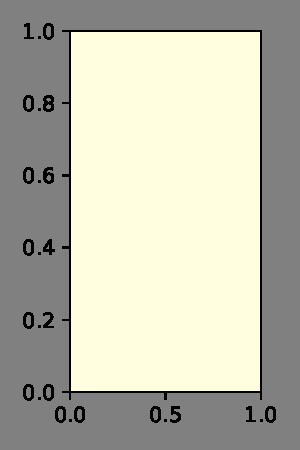
\includegraphics[width = .45\textwidth]{proseplots/figparams.pdf}
\end{center}


The axes object, named \code{ax} by convention, gets more use in most programs. In place of \code{plt.plot()}, you'll use \code{ax.plot()}. Similary, \code{plt.hist()} is replaced with \code{ax.hist()} to create a histogram. If you have experience with the MATLAB interface, you might get reasonably far with the object-oriented style just replacing the \code{plt} prefix on your pyplot functions with \code{ax} to see if you have an equivalent axes method.

This wishful coding won't take you everywhere though. For example, \code{plt.xlim()} is replaced by \code{ax.set_xlim()} to set the $x$-axis view limits. To modfiy the title, \code{plt.title()} is replaced with \code{ax.set_title()} and there is \code{ax.get_title()} simply to get the title. The axes object also happens to have a \code{title} attribute, which is only used to access the title, similar to the \code{get_title()} method. Many matplotlib methods can be classified as \emph{getters} or \emph{setters} like for these title methods. The plot method and its logic is different. Later calls of \code{ax.plot()} don't overwrite earlier calls and there is not the same getter and setter form. There's a \code{plot()} method but no single \code{plot} attribute being mutated. Whatever has been plotted can be retrieved, or gotten (getter'd?), but it's more complicated and rarely necessary. Use the code below to see what happens with two calls of \code{plot()} and two calls of \code{set_title()}. The second print statement demonstrates that the second call of \code{set_title()} overwrites the title attribute, but a second plot does not nullify the first. 

%It's part of the object-oriented construction, which goes beyond our scope.
%\newpage

 
\begin{lstlisting}[language = Python, caption= {[gettersetter.py]}]
x = np.linspace(0,1,2)    (*@\margintext{gettersetter}@*) 
fig, ax = plt.figure(figsize = (8,4)), plt.axes()
ax.plot(x, x)
ax.plot(x, 1 - x)
ax.set_title("My Chart")
print(ax.title)
print(ax.get_title()) # Similar to above line
ax.set_title("My Wholesome Chart")
print(ax.get_title()) # long
\end{lstlisting}

\begin{center}
    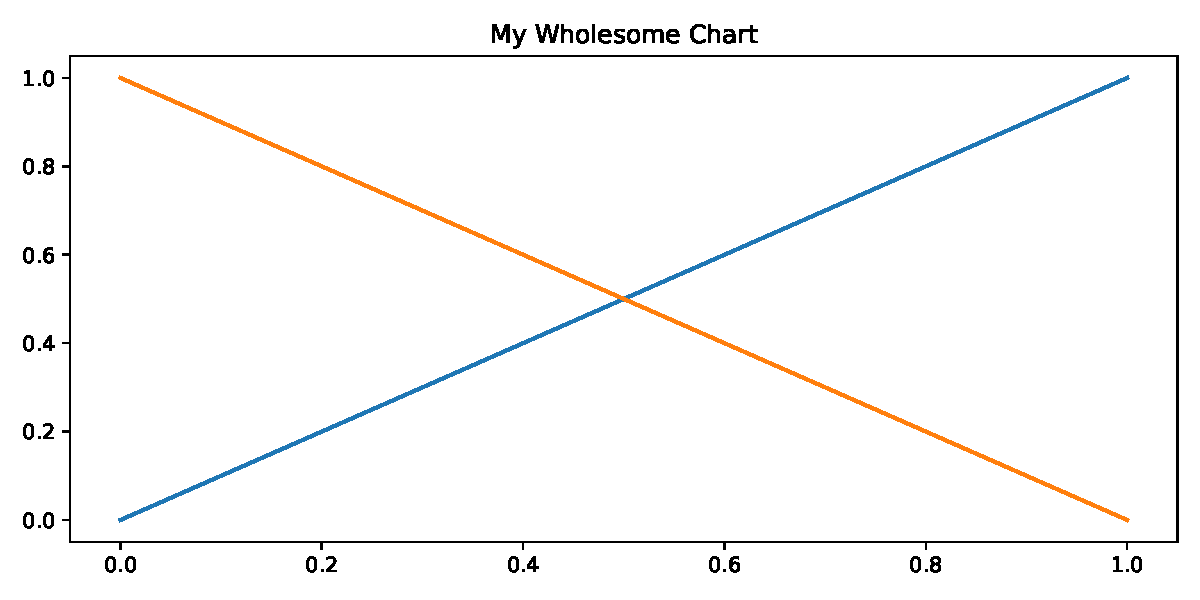
\includegraphics[width = .7\textwidth]{proseplots/gettersetter.pdf}
\end{center}

Axes methods \code{set_xlim()} and \code{get_xlim()} behave just like \code{set_title()} and \code{get_title()}, but note there is no attribute simply accessible with \code{ax.xlim}, so the existence of getters and setters is the more fundamental pattern.\footnote{Getters and setters are thought of as old-fashioned. It's more Pythonic to access attributes directly, but matplotlib doesn't yet support this.}
%https://matplotlib.org/stable/tutorials/intermediate/artists.html?highlight=artist%20tutorial for old fashioned comment

\subsubsection{Mixing the Interfaces}

You can also mix the interfaces. Use \code{plt.gca()} to \emph{g}et the \emph{c}urrent \emph{a}xis. Use \code{plt.gcf()} to \emph{g}et the \emph{c}urrent \emph{f}igure.

\begin{lstlisting}[language = Python, caption={[chart.py]}]
x = np.linspace(0,1,2) 
plt.plot(x,x)
plt.title("My Chart")

ax = plt.gca()
print(ax.title)

ax.plot(x, 1 - x)
ax.set_title('My Wholesome Chart')
print(ax.title)

fig = plt.gcf()
fig.savefig('chart.pdf') # same as plt.savefig
\end{lstlisting}

\begin{center}
    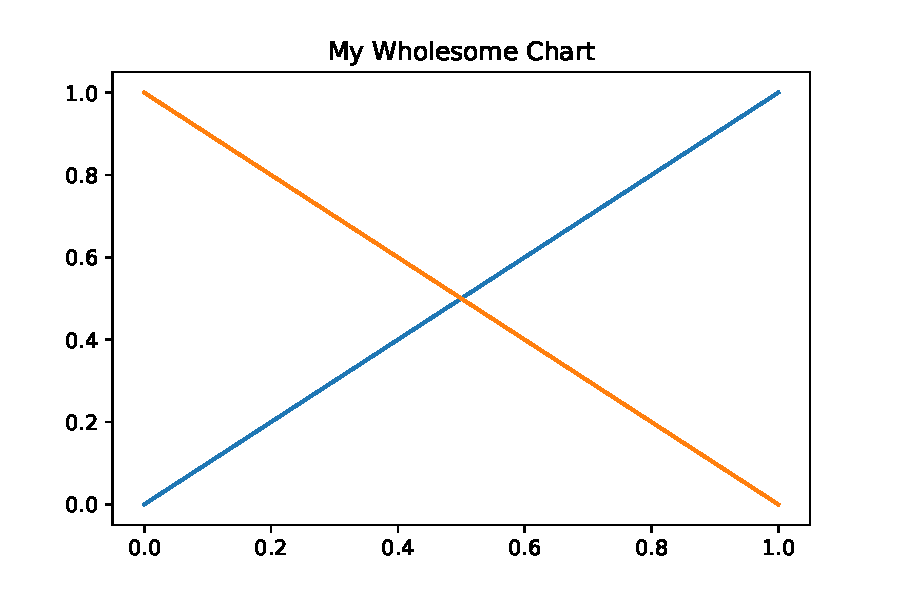
\includegraphics[width = .8\textwidth]{proseplots/chart.pdf}
\end{center}


In the above, we started with MATLAB and then converted to object-oriented. We can also go in the opposite direction as well. We can also mix pandas with MATLAB or OOP-style matplotlib. 

These plots can be mixed with the object-oriented interface. You can use a plot method and specify the appropriate axes object as an argument. Below we import the iris dataset and make a boxplot with a mix of axes methods and then pyplot functions. 

\begin{lstlisting}[language = Python, caption= {[irisbox.py]}]
from sklearn.datasets import load_iris 
data = load_iris()['data']
df = pd.DataFrame(data)

fig, ax = plt.figure(), plt.axes()

df.plot.box(ax = ax)
ax.yaxis.grid(True)
ax.xaxis.grid(False)

plt.tight_layout()
plt.savefig('irisbox.pdf')
\end{lstlisting}

\begin{center}
    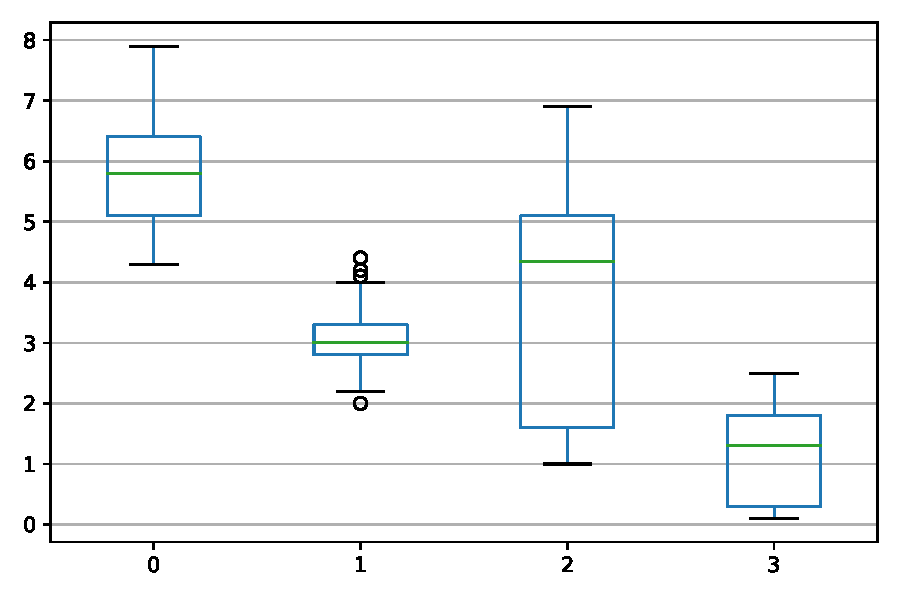
\includegraphics[width = .7\textwidth]{proseplots/irisbox.pdf}
\end{center}



\subsection{Subplots with \code{plt.subplots()}}

You can use \code{subplots()} to create multiple subplots within the figure.

\begin{lstlisting}[language = Python]
# Multiple Subplots
# ax is a tuple for two different axes
fig, ax = plt.subplots(1,2)

# Call plot() on the axis
ax[0].plot(x, np.sin(x))
ax[1].plot(x, np.sin(x), color = 'tomato')

plt.show()
\end{lstlisting}

In the last example above, two subplots are created. If you save this, note this creates a single image file, not one for each subplot. Next, we create a $2\times 2$ grid. Note, when we do this, we must index \code{ax} at two layers. Before, in a $1\times2$, we had one-dimensional indexing. The superfluous second dimension was \emph{squeezed} out by default.\footnote{See the \code{squeeze} parameter in the \link{https://matplotlib.org/3.5.0/api/_as_gen/matplotlib.pyplot.subplots.html}{documentation}.}

\begin{lstlisting}[language = Python]
fig, ax = plt.subplots(2,2)

x = np.linspace(0, 2 * np.pi)
y = np.sin(x)

ax[0,0].plot(x,y)
ax[0,1].plot(x,y, linestyle = 'dashed')
ax[1,0].plot(x,y, linestyle = 'dotted', color = 'black')
ax[1,1].plot(x,y, linewidth = 7)

for ax_ in fig.axes:
    ax_.set_title('Sine Wave')

fig.suptitle("Big Plot", size = 20)
plt.tight_layout()

plt.savefig("subplot_example_2by2.pdf")
\end{lstlisting}

\begin{center}
    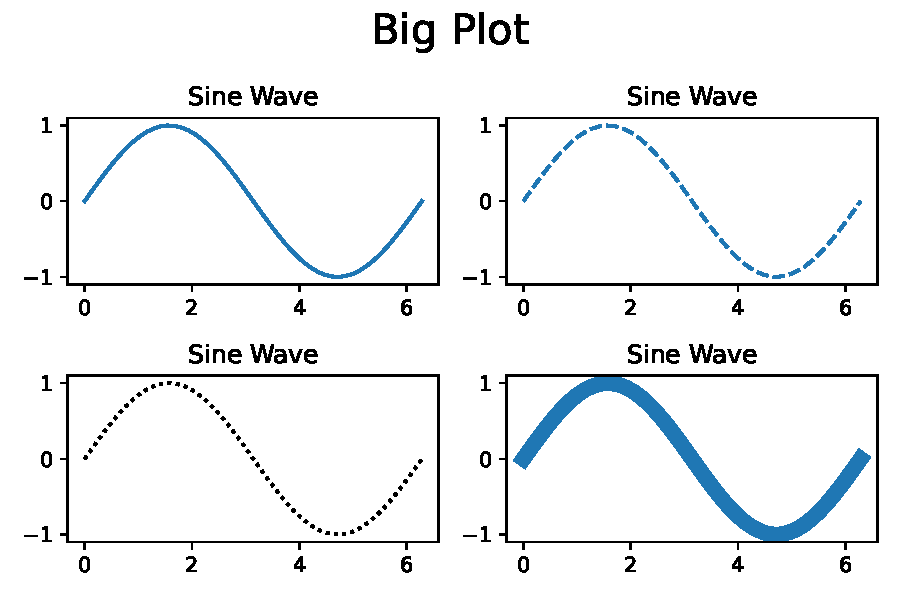
\includegraphics[width = .6\textwidth]{images/subplot_example_2by2.pdf}
\end{center}

% start out with spine_mod -i
% start out with df.melt()
% more with subplots and squeeze
\chapter{Time and Dates}
%\section{Time Series and Datetime}

\noindent \scalebox{0.8}{\textit{Additional reference: \cite{vanderplas2016python} Chapter 3}}


Up to now, we've only encountered dates as strings like \code{independence_day = '1776-07-04'}. This is limited. For example, there are no string operations to add and subtract days. To that end, it is helpful to have new classes for date objects and ways to manipulate those dates, times, and datetimes. The built-in \code{datetime} and \code{dateutil} modules are useful for that. These will only support times since 1 AD. This might disappoint astronomers or anyone else wanting to extend their analysis to years BC. If that's you, you'll have to study the AstroPy \link{https://docs.astropy.org/en/stable/api/astropy.time.Time.html}{Time class}.

\section{Using the \texttt{datetime} module}

The standard import is \code{import datetime as dt}. 

\subsection{Dates and Datetimes}
The two main classes are \code{date} and \code{datetime}. A \code{date} object is created with \code{dt.date(year, month, day)}. \code{datetime} extends this with optional parameters for hour, minute, second, microsecond, timezone information, and \link{https://docs.python.org/3/library/datetime.html\#datetime.datetime.fold}{fold}. 

\begin{lstlisting}
last_lecture1 = dt.date(2022, 5, 2)
last_lecture2 = dt.datetime(2022, 5, 2, 20, 10)

now = dt.datetime.today() # get current date and time
print(now) # local NYC time for me
\end{lstlisting}

You can go back to a date from a datetime with the datetime method \code{date()}. You can get a \code{time} object with the dateime method \code{time()}. 

We won't cover time zones or folds. But on time zones, you should be aware that some datetimes are automatically in local time. In New York City, this comes as a -4 or -5 offset from UTC (coordinated universal time). For more with timezones, use \link{https://pypi.org/project/pytz/}{pytz}. Below is a small taste of pytz for anyone curious. 

\begin{lstlisting}
import pytz

unaware = dt.datetime(2014,2,2) # time zone unaware datetime
aware = pytz.utc.localize(unaware) # sets tzinfo to be UTC without changing the hour
\end{lstlisting}

\subsection{Unix Timestamps}

Beyond strings like \code{'2022-12-25'}, you might also encounter timestamps as integers. That is, you might use \link{https://en.wikipedia.org/wiki/Unix_time}{Unix time}. This is also called POSIX time. These integers give the number of seconds elapsed since 00:00:00 UTC on 1 January 1970 (the Unix epoch). 

These can be converted to datetime objects as shown below. 

\begin{lstlisting}
# UTC
# This gives 1970, 1, 1, 0, 0
dt.datetime.utcfromtimestamp(0)

# Local Time
# This gives 1969, 12, 31, 19, 0 (NYC)
dt.datetime.fromtimestamp(0)

# Can also use dt.date on fromtimestamp
# This gives 1969, 12, 31 (NYC)
dt.date.fromtimestamp(0)
\end{lstlisting}

\subsection{Time Deltas and Relative Deltas}

A \code{timedelta} object is useful for dealing with a duration of time, when subtracting datetimes for example. 


\begin{lstlisting}[language = Python]
class_start = dt.datetime(2020,12,5,12,10,0)
class_end = class_start + dt.timedelta(hours = 1, minutes = 50)

class_duration = class_end - class_start

print(class_duration)
\end{lstlisting}

The \code{seconds} attribute is different than the \code{total_seconds()} method. Can you anticipate the difference?
\begin{lstlisting}
delta = dt.timedelta(days = 1, seconds = 100)

print(delta.seconds)
print(delta.total_seconds())
\end{lstlisting}

But what if we just want the next month? We can't use a single timedelta that takes us from February 1st to March 1st and also from April 1st to May 1st. For this, we need a \code{relativedelta} from \code{dateutil}.

\begin{lstlisting}
from dateutil.relativedelta import relativedelta

date = dt.date(2019, 12, 9)
other_date = date + relativedelta(months = 2)
print(other_date)

# Consider how this works with leap year
next_year1 = date + relativedelta(years = 1)
next_year2 = date + dt.timedelta(days = 365)
\end{lstlisting}



\subsection{Date Strings}

The datetime \code{strptime} method is very useful in string conversion. It works with a date string as its first argument and a \link{https://docs.python.org/3/library/datetime.html\#strftime-and-strptime-format-codes}{format} as a second argument. 

For example, \code{dt.datetime.strptime('2020-01-01', '\%Y-\%m-\%d')} returns a datetime object for January 1st, 2020. 

Above, the string \code{'\%Y-\%m-\%d'} is a date format code. Here are some common format codes, applied to Sunday January 30, 2000, 11:59PM, local to Louisville, Kentucky. These can all be verified with \code{pd.Timestamp(year = 2000, month = 1, day = 30, hour = 23, minute = 59, tz = 'America/Kentucky/Louisville').strftime()}.

\begin{center}
\begin{small}
{\setlength{\tabcolsep}{2em}
\begin{tabular}{ll}
\toprule
Code & Output/Example \\
\midrule
\code{'\%Y'} & 4-Digit Year \\
\code{'\%m'} & Month Number \\
\code{'\%d'} & Day of Month \\
\code{'\%B'} & Month Name \\
\code{'\%H'} & 24-Hour Clock Hour \\
\code{'\%M'} & Minute \\
\code{'\%H'} & 12-Hour Clock Hour \\
\code{'\%p'} & AM or PM \\
\code{'\%A'} & Day of Week \\
\code{'\%Z'} & Timezone Name \\
\code{'\%Y-\%m'} &   \code{'2000-01'}\\
\code{'\%Y\/\%m/\%d'} & \code{'2000/01/30'}\\
\code{'\%B \%y'} & \code{'January 00'}\\
\code{'\%H:\%M \%Z'} & \code{'23:59 EST'} \\
\code{'\%A \%I\%p'} & \code{'Sunday 11PM'}\\
\bottomrule
\end{tabular}}
\end{small}
\end{center}

A more complete list of format codes can be found at \link{https://strftime.org}{strftime.org}. Codes that generate actual names, like \code{'\%A'} or \code{'\%B'}, can be made lowercase to produce an abbreviated name. Notice that these formats create zero-padded numbers like \code{'07'} instead of \code{'7'}. On Mac or Linux, padding can be eliminated with the \code{'-'} modifier, using \code{'\%-H'} or \code{'\%-m'}
instead of \code{'\%H'} or \code{'\%m'} for example. On Windows, use \code{'#'}.


\subsubsection{Dateutil}

Dateutil offers, among other things, a details-free parser (you don't have to specify a format code).

\begin{lstlisting}[language = Python]
from dateutil import parser
date = parser.parse("9th of December, 2019")
print(date)
\end{lstlisting}



\subsection{Pandas and Numpy}
Pandas offers an efficient \code{Timestamp} object and NumPy offers an efficient \code{datetime64}. For NumPy, the tradeoff is they are less flexible than datetime objects. Pandas offers something closer to the best of both worlds.

Notice the accessing a NumPy array from a Series will convert datetime objects into NumPy's datetime64. 

\begin{lstlisting}[language = Python]
ser = pd.Series([dt.datetime.today()])
date = ser.values[0]
print(date)

# date + dt.timedelta(days = 1)  # error
\end{lstlisting}

Here, we parse a date into a Pandas Timestamp and use a datetime timedelta. 

\begin{lstlisting}[language = Python]
date = pd.to_datetime("4th of July, 2015")
print(date)
print(type(date))

date + dt.timedelta(days = 1) # Works
\end{lstlisting}


In pandas, we can also parse dates when reading in a CSV, using the \code{parse_dates} parameter in \code{pd.read_csv()}. A string for a single column or a list for multiple columns are both valid arguments. 

\section{Analysis}

\begin{lstlisting}[language = Python]
dates = pd.date_range(start='2020-12-05', end='2021-12-05', freq='1D')

df = pd.DataFrame(index = dates)

df['stock_price'] = range(len(dates)) + np.random.normal(0,10,len(dates))
plt.plot(df['date'], df['stock_price'])
plt.show()


## Rolling Function

data = df.stock_price.rolling(30, center = True)
data.mean().plot()
plt.show()
\end{lstlisting}

Try it with other window sizes. 

\begin{lstlisting}[language = Python]
data = df.stock_price.rolling(365, center = True)
data.mean().plot()
plt.show()

data = df.stock_price.rolling(100, center = True)
data.mean().plot()
plt.show()
\end{lstlisting}

\subsection{Application 1}
Load the NYC taxi data and look at the distribution of ride lengths. 

\begin{lstlisting}[language = Python]
df = pd.read_csv('nyc_data.csv')

df.head(1)
\end{lstlisting}

\begin{lstlisting}[language = Python]
df['pickup_datetime'] = pd.to_datetime(df['pickup_datetime'])
df['dropoff_datetime'] = pd.to_datetime(df['dropoff_datetime'])

df['duration'] = df['dropoff_datetime'] - df['pickup_datetime']

# Make histogram with logarithmic y axis
df['duration'].dt.total_seconds().hist(log = True)
\end{lstlisting}


\subsection{Application 2}

Load the \texttt{ATUS\_activity\_2019.csv} dataset. Create a new datetime time object column from the \texttt{TUSTARTTIM} column.

\subsubsection{Method 1}
\begin{lstlisting}[language = Python]
import datetime
import pandas as pd

df = pd.read_csv("ATUS_activity_2019.csv")

# Parse the time
df['time_col'] = df['TUSTARTTIM'].map(lambda x: dt.datetime.strptime(x, "%H:%M:%S"))

# This sets everything to a datetime object from January 1900
# Convert to time with the time method

df['time_col'] = df.time_col.map(lambda x: x.time())
\end{lstlisting}


\chapter{Python for Excel}
\noindent \scalebox{0.8}{\textit{Reference: \cite{zumstein2021}}}
\smallskip

Excel (or Google Sheets) is unavoidable if you work with enough people, especially ThinkPad people. You will want to deliver a spreadsheet to a stakeholder, not a Python script. And that spreadsheet will be received better if it's well formatted. That means we're not talking about a CSV file fresh from \code{df.to_csv()}. In this chapter, we'll use Python to do the following.

\begin{enumerate}
    \item Save to individual sheets in a larger workbook.
    \item Read in individual sheets as dataframes.
    \item Apply cell formatting.
    \item Apply filters.
    \item Insert plots in a sheet.
\end{enumerate}

\noindent If you're in this class, you're way too smart to do these tasks by pointing and clicking in a GUI. We'll use pandas and \link{https://openpyxl.readthedocs.io/en/stable/}{OpenPyXL}.% and \link{https://xlsxwriter.readthedocs.io/}{XlsxWriter}. 

\section{Pandas}

Pandas comes with the \code{read_excel()} function and the \code{to_excel()} method. Below, we use these most basically. 

\begin{lstlisting}
df = pd.DataFrame({'a': [0]})

# Save to excel file
df.to_excel("mwe.xlsx", index = None)

# Clear df from memory
del df

# Read
df = pd.read_excel("mwe.xlsx")
\end{lstlisting}

We go into more detail in this section. However, pandas is limited. Separate reader and writer packages are useful for including charts, changing formatting, etc. 

\subsection{Reading}

Above, \texttt{mwe.xlsx} is the simplest and most well-behaved kind of Excel file you can encounter. There are not multiple sheets and the data begins in cell A1. Often, you'll receive an Excel file with multiple sheets and with some formatting that, to a Python user, is wonky. Reading in the right sheets is priority number one. You can use the \code{sheet_name} parameter to specify the sheet you want to use, by name or index. If you pass a list of sheet names, \code{read_excel()} returns a dictionary with the DataFrames as values and sheet names as the keys. Use \code{sheet_name = None} to load all of the sheets. 

Maybe the first row and first column are blank, in which case the data begins in cell B2. 
Use \code{skiprows} and \code{usecols} to specify the cell range you want to use. These and other parameters are described in Table 7-1 in \cite{zumstein2021}. The additional parameters are mostly useful for data cleaning, so you can have that done in the \code{read_excel()} call instead of in additional lines of code. 

\subsection{Writing}

As with \code{read_excel()}, \code{to_excel()} includes a \code{sheet_name} parameter. However, this can't be used to add multiple sheets to a single Excel file. The method doesn't \emph{add} a new sheet to an existing file, it merely writes the Excel file from scratch, with a single sheet named according to \code{sheet_name}. 

\begin{lstlisting}
df = pd.DataFrame({'a': [0]})

# creates mwe.xlsx with one sheet called A
df.to_excel("mwe.xlsx", index = None, sheet_name = 'A')

# overwrites mwe.xlsx, one sheet called B
df.to_excel("mwe.xlsx", index = None, sheet_name = 'B')
\end{lstlisting}


To add multiple DatFrames to different sheets (or even within the same sheet), you need to use the \code{ExcelWriter} class. Below, we use \code{ExcelWriter} as a \emph{context manager}, using a \code{with} statement. 

\begin{lstlisting}
df_a = pd.DataFrame({'a': [0]})
df_b = pd.DataFrame({'b': [1]})

with pd.ExcelWriter('multi_sheet.xlsx') as writer:
    df_a.to_excel(writer, sheet_name = 'A', index = None)
    df_b.to_excel(writer, sheet_name = 'B', index = None)
\end{lstlisting}

The additional parameters for \code{to_excel()} deserve some attention, because they aren't as easily replaced by other lines of code. Neglecting them creates more work for you in Excel, and our objective is to avoid that. Some parameters are described in Table 7-2 in \cite{zumstein2021} and in the \link{https://pandas.pydata.org/docs/reference/api/pandas.DataFrame.to_excel.html}{official documentation}. 

\begin{center}
\begin{small}
{\setlength{\tabcolsep}{2em}
\begin{tabular}{ll}
\toprule
Parameter & Description \\
\midrule
\code{startrow} & First row where the DataFrame is written (using zero-based indexing) \\
\code{startcol} & First column where the DataFrame is written (using zero-based indexing) \\
\code{freeze_panes} & Takes a tuple for the number of rows and columns to freeze. \\
& Passing \code{(1,2)} freezes the first row and the first two columns. \\
\bottomrule
\end{tabular}}
\end{small}
\end{center}

\section{OpenPyXL}

\paragraph{Installation:}
OpenPyXL is useful for reading, writing, and editing Excel files. If you need to install it, run \texttt{conda install -c anaconda openpyxl} or \texttt{pip install openpyxl} in the terminal. %We'll also need Pillow to include images. Thus, \texttt{conda install -c anaconda pillow} or \texttt{pip install pillow}.

Remember, there are three levels to an Excel file: the workbook, the worksheet, and the individual cells. The workbook is the entire file and all the sheets (or tabs). The worksheet is an individual tab. And a cell is the entry at a specific coordinate in a worksheet. OpenPyXL has classes \code{Workbook}, \code{Worksheet}, and \code{Cell} for each of these. 

\subsection{Reading}

Use \code{load_workbook()} to read in data and specify \code{data_only = True} to read in the cell values instead of the cell formulas.

\begin{lstlisting}
import pandas as pd
import openpyxl
import datetime as dt

# Workbook object
book = openpyxl.load_workbook('multi_sheet.xlsx', data_only = True)

# get a list of all sheet names
print(book.sheetnames)

# Worksheet objects
sheet_a = book['A']
sheet_b = book['B']

# Get dimensions
print(sheet_a.max_row, sheet_a.max_column)

# Cell object
cell = sheet_a['A1']
print(cell.value)
\end{lstlisting}

\subsection{Writing}


We write a DataFrame to an Excel .xlsx file using the functionality provided directly in OpenPyXL, making use of \code{dataframe_to_rows}.\footnote{\cite{zumstein2021} provides a module \link{https://github.com/fzumstein/python-for-excel/blob/1st-edition/excel.py}{excel.py}. It's handy for going back and forth between OpenPyXL and other Excel packages. However, it doesn't play that well with index and header values.} The process is as follows. 

\begin{enumerate}
    \item Create a Workbook instance.
    \item Access a Worksheet. Below we use the \code{active} attribute to get the currently active sheet.
    \item Append data to the bottom of the sheet using the Worksheet \code{append()} method. 
    \item Save the Workbook using the \code{save()} method.
\end{enumerate}

\begin{lstlisting}
from openpyxl.utils.dataframe import dataframe_to_rows

wb = openpyxl.Workbook()
ws = wb.active

for r in dataframe_to_rows(df, index=True, header=True):
    ws.append(r)

wb.save("pandas_openpyxl.xlsx")
\end{lstlisting}

This includes the index and header (column name) values given the parameters in \code{dataframe_to_rows}. Our Excel file includes a sheet as shown below. 

\begin{center}
    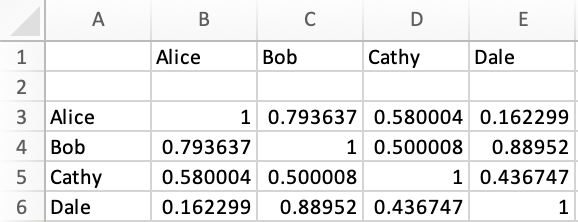
\includegraphics[width = 0.7\textwidth]{images/excel_ss1.png}
\end{center}

\noindent If we had simply used \code{df.to_excel('filename.xlsx')}, we'd end up with the below. 

\begin{center}
    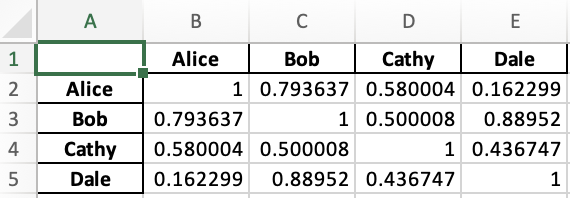
\includegraphics[width = .7\textwidth]{images/excel_pandas_save.png}
\end{center}

\noindent Why the empty row when using OpenPyXL? I'm not sure.\footnote{See the \link{https://openpyxl.readthedocs.io/en/stable/pandas.html?highlight=dataframe\#working-with-pandas-dataframes}{documentation here} if you'd like to delve further on your own.} The \code{dataframe_to_rows()} function finds an empty row somewhere, somehow. We can avoid appending this to our worksheet by modifying the for-loop, as is done below. 

\begin{lstlisting}[label = {lst:wb}]
from openpyxl.utils.dataframe import dataframe_to_rows

wb = openpyxl.Workbook()
ws = wb.active

for r in dataframe_to_rows(df, index=True, header=True):
    print(r)
    if r != [None]:
        ws.append(r)

wb.save("pandas_openpyxl.xlsx")
\end{lstlisting}


\subsection{Styles}

Styles and formatting can be applied, but only one cell at a time. Accordingly, we need to learn more about the \code{Cell} class.\footnote{\link{https://openpyxl.readthedocs.io/en/stable/api/openpyxl.cell.cell.html}{\code{Cell} documentation here.}} A specific cell can be accessed by indexing a worksheet with the appropriate coordinate, \code{ws['A1']} for example. Cell ranges can be accessed as might be done in Excel. Columns A-C can be obtained with \code{ws['A:C']}. Rows 3-5 can be accessed with \code{ws[3:5]}. Note cell ranges are just tuples of cells. There is also a \code{iter_rows()} worksheet method, returning a generator for iteration. 

Below are some basic \code{Cell} attributes.

\begin{center}
\begin{small}
{\setlength{\tabcolsep}{2em}
\begin{tabular}{ll}
\toprule
Attribute & Description \\
\midrule
\code{coordinate} & The Excel coordinate of the cell (e.g. \code{'B2'}) \\
\code{column} & Column number of the cell (one-based) \\
\code{row} & Row number of the cell (one-based) \\
\code{column_letter} & Column letter of the cell (e.g. \code{'B'} or \code{'AA'}) \\
\code{value} & Data value of the cell \\
\code{is_date} & Boolean value \\
\bottomrule
\end{tabular}}
\end{small}
\end{center}

There are \code{Cell} style attributes you might use to inspect and to overwrite the cell font, border, alignment, fill, and number format. To set these, use the \code{openpyxl.styles} submodules. For example, to set the cell alignment, write \code{ws['C8'].alignment = openpyxl.styles.alignment.Alignment(horizontal = 'center')}.

\begin{center}
\begin{small}
{\setlength{\tabcolsep}{2em}
\begin{tabular}{ll}
\toprule
Attribute & \code{openpyxl.styles} submodule and class  \\
\midrule
\code{font} & \code{Font} \\
\code{border} & \code{borders.Side} and \code{borders.Border} \\
\code{alignment} & \code{alignment.Alignment} \\
\code{fill} & \code{fills.PatternFill} \\
\code{number_format} & N/A (use a string) \\
\bottomrule
\end{tabular}}
\end{small}
\end{center}

The final attribute listed above, \code{number_format}, is set with a string. Available format examples can be found in the \link{https://openpyxl.readthedocs.io/en/stable/_modules/openpyxl/styles/numbers.html}{OpenPyXL documentation} and the \link{https://support.microsoft.com/en-us/office/review-guidelines-for-customizing-a-number-format-c0a1d1fa-d3f4-4018-96b7-9c9354dd99f5}{Microsoft documentation} provides further detail. Below are a few formats and their Excel output.\footnote{Access the \link{https://docs.google.com/spreadsheets/d/10ME-F1CMkeUCXRyoUj3EYsKFvfyyJe61/edit?usp=sharing&ouid=102598671780190894865&rtpof=true&sd=true}{spreadsheet here}.}


\begin{center}
    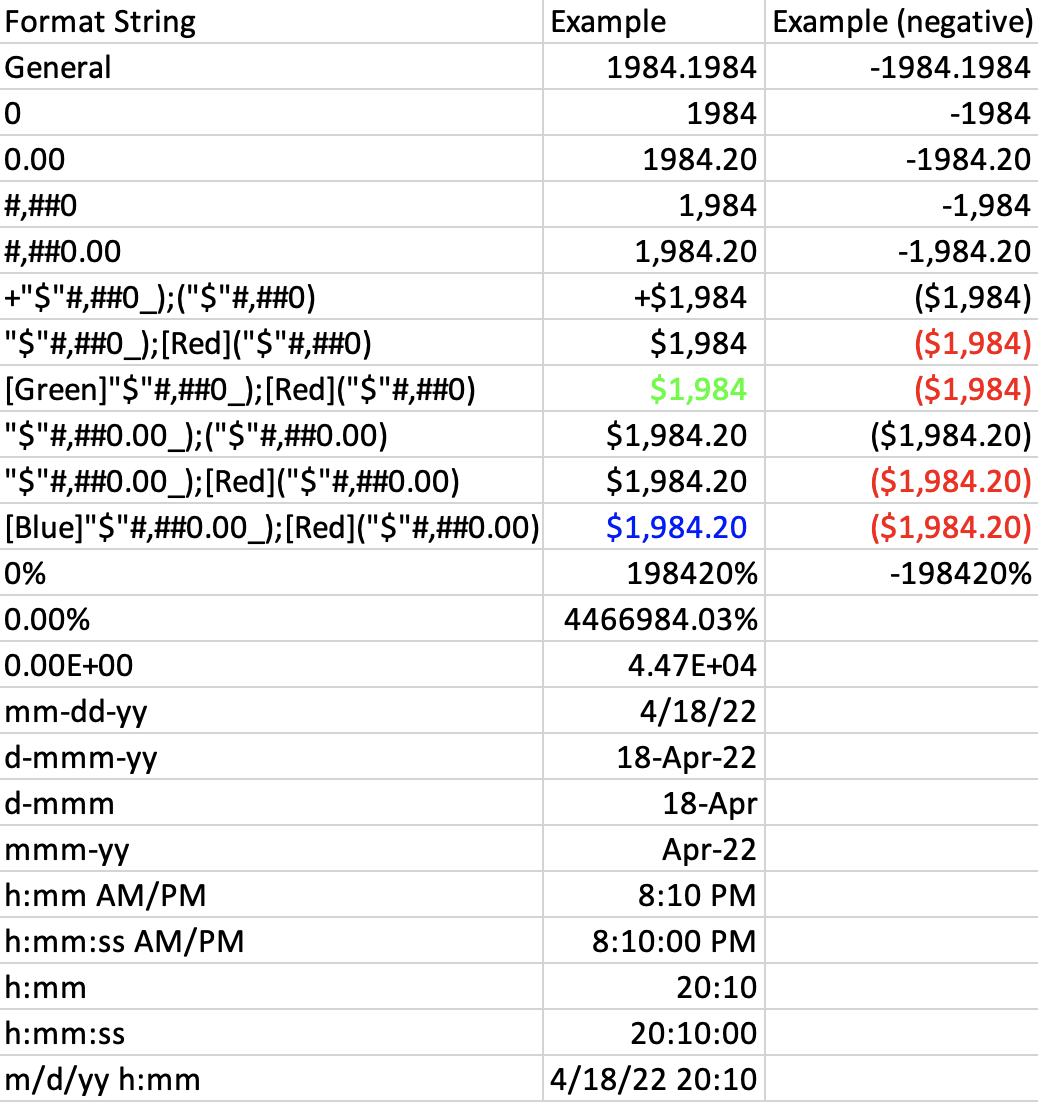
\includegraphics[width = .8\textwidth]{images/excel_formats2.png}
\end{center}

The above is created with this code. 

\begin{lstlisting}
import openpyxl

formats = ['General',
     '0',
     '0.00',
     '#,##0',
     '#,##0.00',
     '+"$"#,##0_);("$"#,##0)',
     '"$"#,##0_);[Red]("$"#,##0)',
     '[Green]"$"#,##0_);[Red]("$"#,##0)',
     '"$"#,##0.00_);("$"#,##0.00)',
     '"$"#,##0.00_);[Red]("$"#,##0.00)',
     '[Blue]"$"#,##0.00_);[Red]("$"#,##0.00)',
     '0%',
     '0.00%',
     '0.00E+00',
     'mm-dd-yy',
     'd-mmm-yy',
     'd-mmm',
     'mmm-yy',
     'h:mm AM/PM',
     'h:mm:ss AM/PM',
     'h:mm',
     'h:mm:ss',
     'm/d/yy h:mm']

wb = openpyxl.Workbook()
ws = wb.active

ws['A1'] = 'Format String'
ws['B1'] = 'Example'
ws['C1'] = 'Example (negative)'
for key, fmt in enumerate(formats):
    
    coord1 = 'A{}'.format(key + 2)
    coord2 = 'B{}'.format(key + 2)
    coord3 = 'C{}'.format(key + 2)
    
    # plain format string
    ws[coord1].value = fmt
    
    # set a date or numeric value and apply format
    if key > 11:
        ws[coord2].value = dt.datetime(2022,4,18,20,10)
    else:
        ws[coord2].value = 1984.1984
        ws[coord3].value = -1984.1984
        ws[coord3].number_format = fmt
    ws[coord2].number_format = fmt

wb.save("openpyxl_formats.xlsx")
\end{lstlisting}

\noindent This leaves \link{https://openpyxl.readthedocs.io/en/stable/api/openpyxl.styles.fonts.html?highlight=fonts\#openpyxl.styles.fonts.Font}{fonts}, \link{https://openpyxl.readthedocs.io/en/stable/api/openpyxl.styles.borders.html?highlight=border\#openpyxl.styles.borders.Border}{borders}, \link{https://openpyxl.readthedocs.io/en/stable/api/openpyxl.styles.alignment.html?highlight=alignment\#openpyxl.styles.alignment.Alignment}{alignment}, and \link{https://openpyxl.readthedocs.io/en/stable/api/openpyxl.styles.fills.html?highlight=patternfill\#module-openpyxl.styles.fills}{fills} to be explored. 

Here is an example with the Excel result further below. 

\begin{lstlisting}
import openpyxl
import openpyxl.styles as osty
wb = openpyxl.Workbook()
ws = wb.active

words = 'My cup runneth over.'.split(" ")
letters = 'ABCD'
for l, s in zip(letters, words):
    ws['{}1'.format(l)].value = s
    
ws['A1'].font = osty.Font('Times New Roman', bold = True, color = '006400')

ws['B1'].alignment = osty.alignment.Alignment(horizontal = 'right', 
                                              vertical = 'top', 
                                              textRotation = 30)

ws['C1'].fill = osty.fills.PatternFill(fgColor = 'FFFFE3', 
                                       fill_type = 'solid')

medium = osty.borders.Side(border_style = 'medium',
                           color = 'FF0000')
dotted = osty.borders.Side(border_style = 'dotted',
                           color = '87E0FF')
ws['D1'].border = osty.borders.Border(top = medium, 
                                         bottom = medium,
                                         left = dotted,
                                         right = dotted)

wb.save("openpyxl_cup.xlsx")
\end{lstlisting}


\begin{center}
    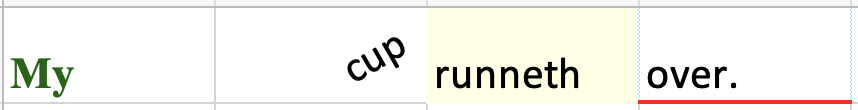
\includegraphics[width = .58\textwidth]{images/cup_runneth.png}
\end{center}

The above uses \code{PatternFill}. There's also \code{GradientFill}, used below. I'm not sure anyone has a use for it. Nonetheless: 

\begin{lstlisting}
wb = openpyxl.Workbook()
ws = wb.active

strings = ['Every man is important if he loses his life;',
         'and every many is funny if he loses his hat and has to run after it.']

for key, s in enumerate(strings):
    ws['A{}'.format(key+1)].value = s

for cell in ws['A']:
    cell.font = osty.Font('Times New Roman', bold = True)

ws['A1'].fill = osty.fills.GradientFill(stop = ['1D97C1', 'FFFFFF'])
ws['A2'].fill = osty.fills.GradientFill(stop = ['FFFFFF', '008080'], degree = 90)

wb.save("openpyxl_chesterton.xlsx")
\end{lstlisting}

\begin{center}
    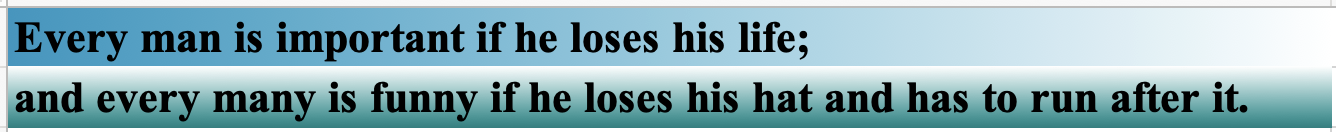
\includegraphics[width = .8\textwidth]{images/excel_chesterton.png}
\end{center}

\subsubsection{Conditional Formatting and Filtering}

Next, we consider conditional formatting. In my experience, the vast majority of any Excel formatting I did was applying a filter and conditional formatting. Below, we take a DataFrame with cosine similarities and send it to a formatted Excel file. 

\begin{lstlisting}
from openpyxl.formatting.rule import ColorScaleRule
import numpy as np
np.random.seed(1)

# Data Generation
a = np.random.rand(n, n)
a = np.triu(a, k = 1) + np.triu(a).T
similarities = a - np.diag(np.diag(a)) + np.diag(np.ones(n))

# Send to DataFrame with index and headers
names = ['product{:0>2}'.format(x) for x in range(n)]
df = pd.DataFrame(similarities, index = names, columns = names)

# Create book and sheet
book = openpyxl.Workbook()
ws = book.active
ws.title = 'Product Similarities'

# Send data to worksheet
for r in dataframe_to_rows(df, index=True, header=True):
    if r != [None]:
        ws.append(r)
        
# Create and apply color rule
rule = ColorScaleRule(start_type='percentile', start_value=10, start_color='ea9999', # red
                       mid_type='percentile', mid_value=50, mid_color='FFFFFF', # white 
                       end_type='percentile', end_value=90, end_color='b6d7a8') # green
ws.conditional_formatting.add('A1:AP42', rule)

# Add Filter over entire spreadsheet
ws.auto_filter.ref = ws.calculate_dimension()

book.save("similarities.xlsx")
\end{lstlisting}


\begin{center}
    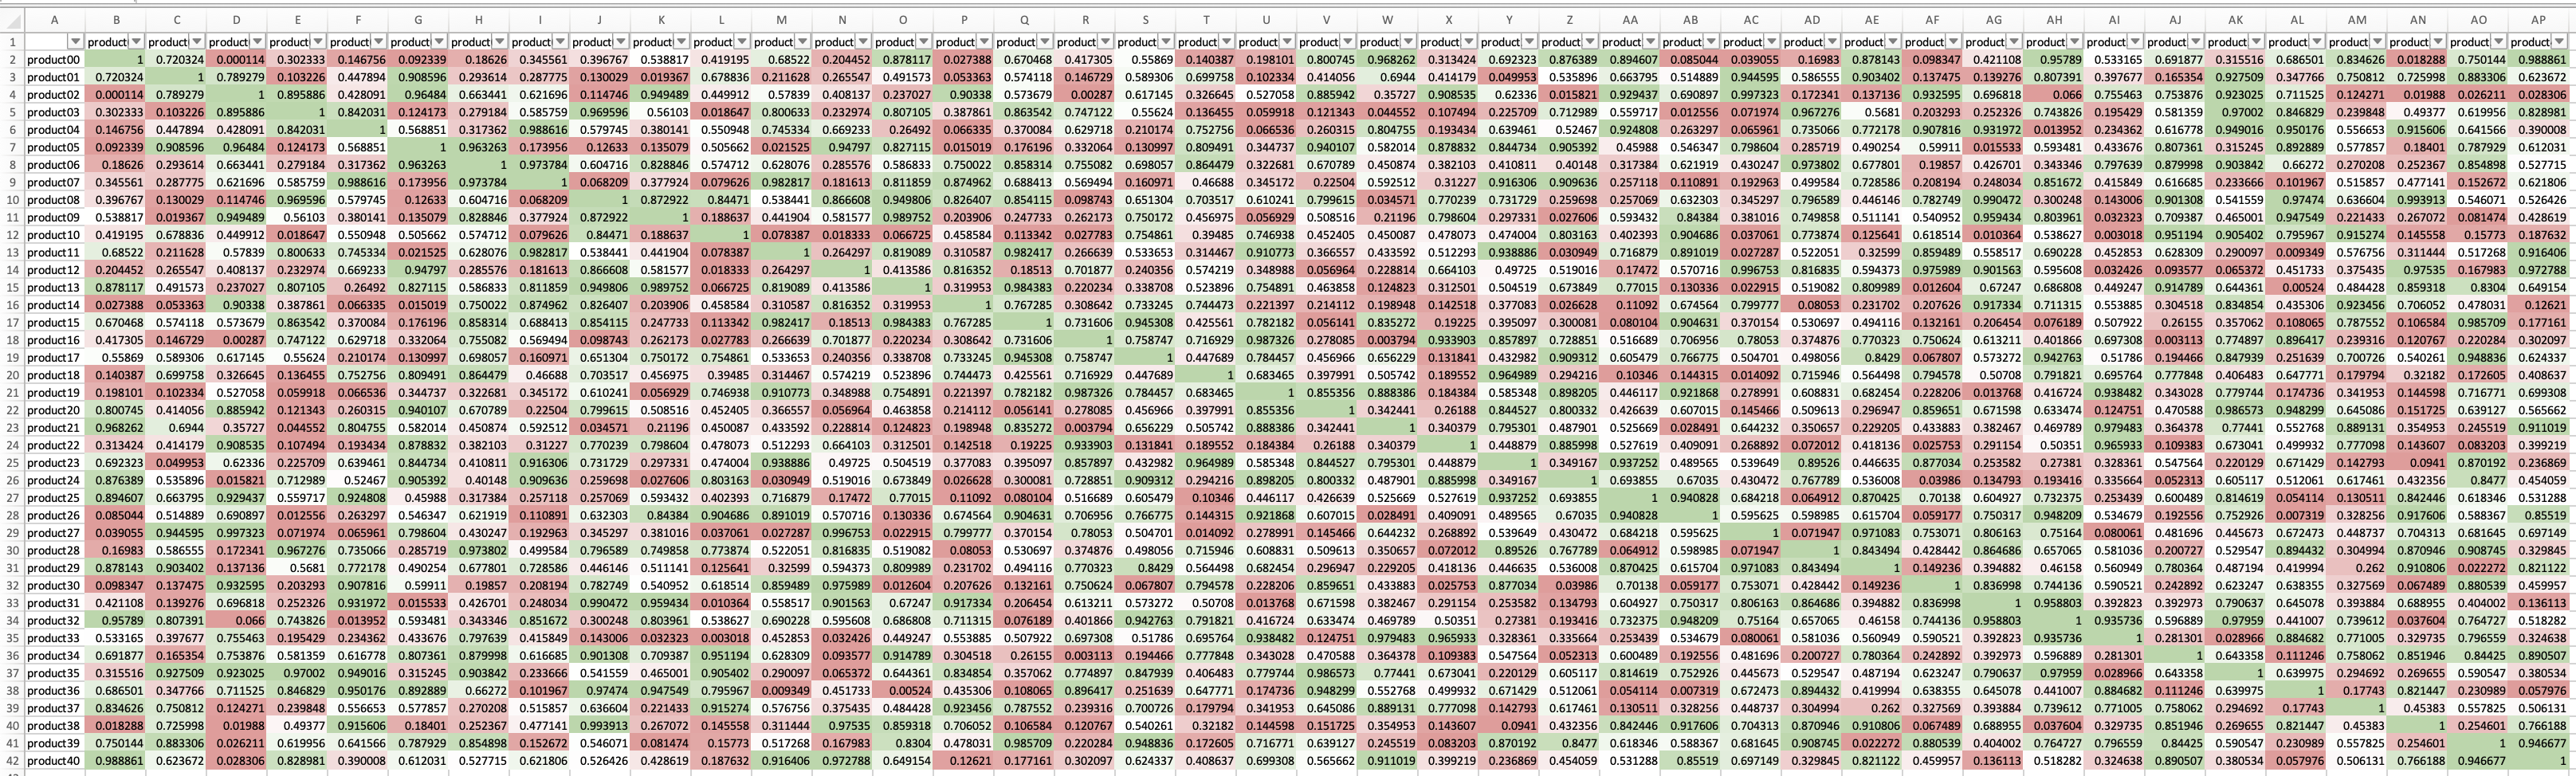
\includegraphics[width = .95\textwidth]{images/similarities.png}
\end{center}



\subsection{Inserting Charts}

Next, we'll add a bar chart using OpenPyXL. See \cite{zumstein2021} Chapter 9 for adding matplotlib images to an Excel file. It's better to include an actual Excel chart as the Excel file user can make further modifications. 



\begin{lstlisting}
#https://openpyxl.readthedocs.io/en/latest/charts/bar.html
from openpyxl import Workbook
from openpyxl.chart import BarChart, Reference

wb = Workbook(write_only=True)
ws = wb.create_sheet()

rows = [ 
        ["Program", 'Wins'],
        ['Kansas', 2357],
       ['Kentucky', 2353],
       ['North Carolina', 2323],
       ['Duke', 2246] ]

for row in rows: #bball_data.reset_index().to_numpy():
    ws.append(row)


chart = BarChart(varyColors = True)
chart.type = "col"
#chart.style = 11
chart.title = "Programs with Most Wins (NCAA Men's Basketball)"
chart.y_axis.title = 'Wins'
chart.x_axis.title = 'Program'

chart.legend = None
data = Reference(ws, min_col=2, min_row=1, max_row=5, max_col=2)
cats = Reference(ws, min_col=1, min_row=2, max_row=5)

chart.add_data(data, titles_from_data=True)
chart.set_categories(cats)

ws.add_chart(chart, "D4")

wb.save("basketball.xlsx")
\end{lstlisting}


We get output like this. 

\begin{center}
    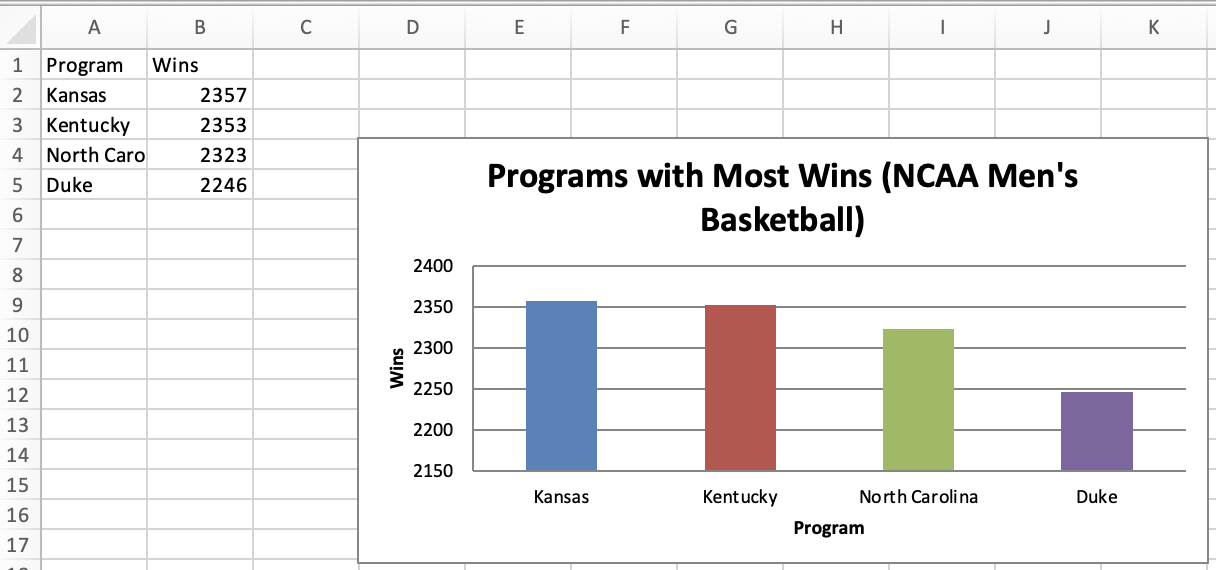
\includegraphics[width = .8\textwidth]{images/basketball_excel.png}
\end{center}

\chapter{Applications}
\section{Inference and Experiments}

In this section, we put our skills together to analyze an A/B test. We'll use pandas, NumPy, and just a bit of statsmodels and SciPy. But first, here's some motivation for why A/B tests are important and to create more student demand for the causal inference course I want to teach. 

\subsection{Motivation/Soapbox}
Any economic or behavioral model proposes to describe the Data Generating Process (DGP), or whatever is really driving the outcomes we see in our non-experimental data. That is, we want to work out if $X$ causes $Y$ or $X$ and $Y$ have a common cause and the association between them is spurious. What would you say if you (plausibly) analyzed data that showed people wearing winter hats are colder than people not wearing winter hats? This is all to say that questions of causality are fraught with issues of bias. Hence the oft-repeated directive \link{https://hbr.org/2021/11/leaders-stop-confusing-correlation-with-causation}{not to confuse correlation with causality}.

The diagrams below depict two different causal models. Suppose you work for a business with a subscription model. It might be Duolingo, Peloton, Netflix, etc. There is normal activity, which is simply using the product and there is social engagement, which might be liking or sharing posts on social media. A product manager might want to know the business impact of social engagement, and both models might create the same correlations between social and retention. \link{https://hbr.org/2018/12/what-great-data-analysts-do-and-why-every-organization-needs-them}{A great analyst} is sensitive to the idea that correlations are not proof of a causal relationship.

\begin{center}
    
    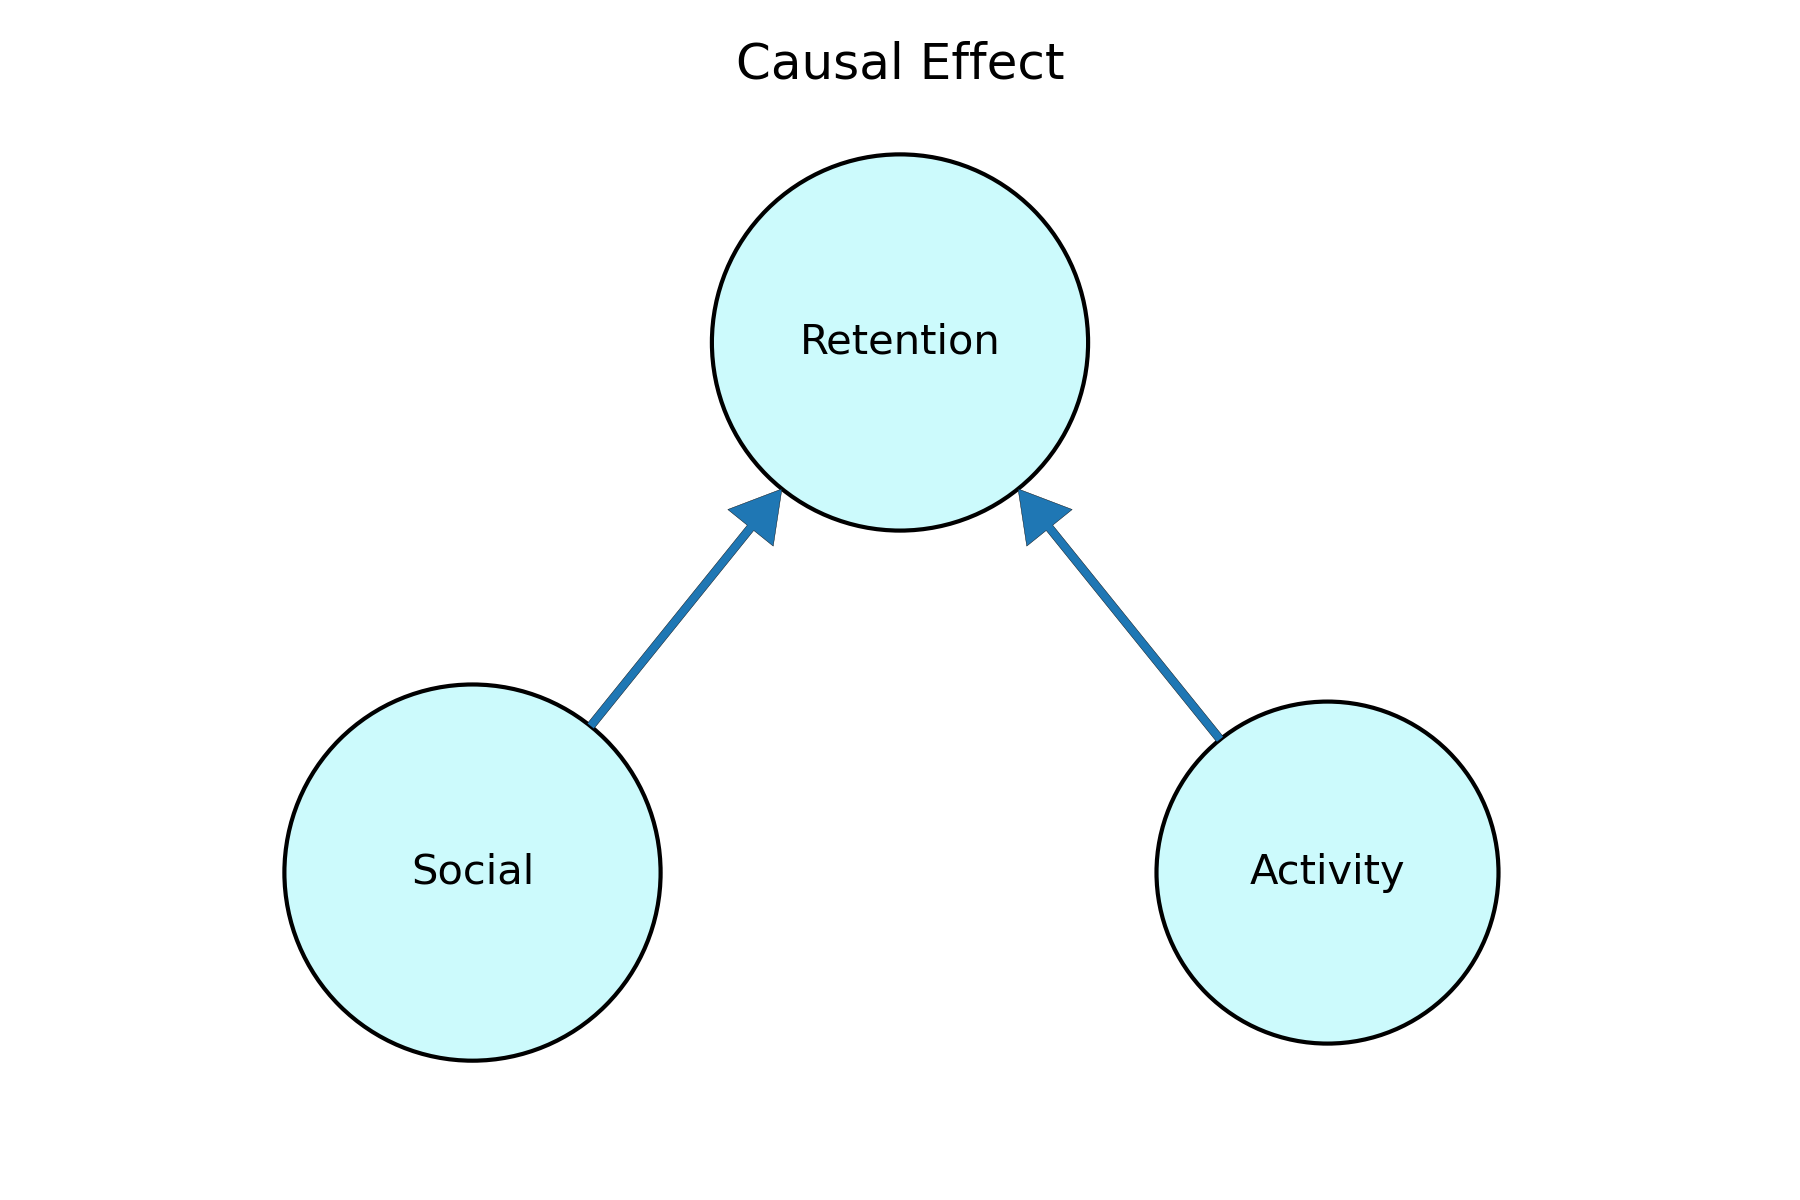
\includegraphics[width =0.48\textwidth]{images/causal1.png} 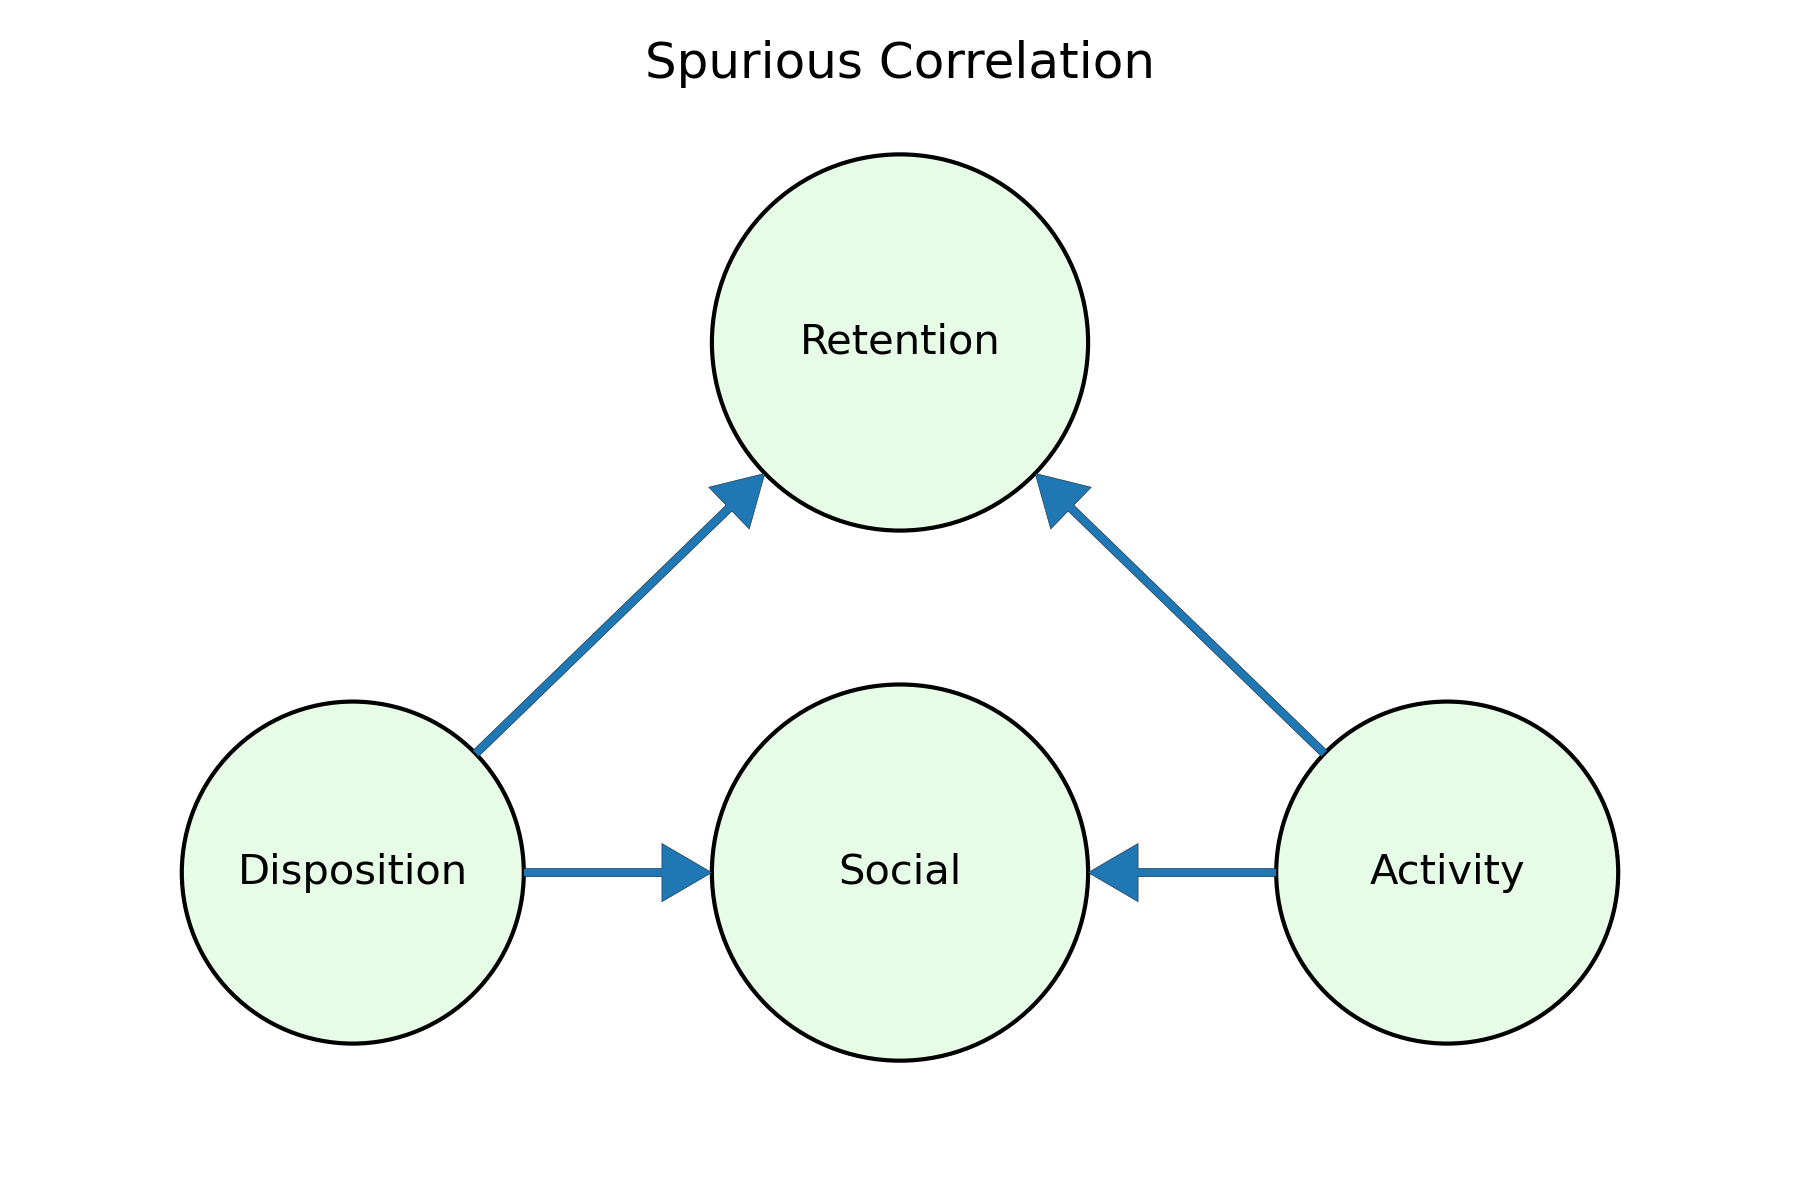
\includegraphics[width = 0.48\textwidth]{images/spurious.png}
\end{center}

On the left, social engagement has a direct effect on the retention outcome. On the right, social engagement has no effect on the retention outcome. However, as we verify in the simulation below, both can produce the same regression output. We'll use OLS for simplicity.  

We regress retention on social engagement and activity, first with data generated by the causal effect process (\code{y1}), then the spurious correlation process (\code{y2}).

\begin{lstlisting}
import statsmodels.api as sm
import pandas as pd

n = 1000
noise = np.random.normal(0, .1, size = n)

# for causal model
activity = np.random.normal(size = n)
social = np.random.normal(size = n)
intercept = np.ones(n)
disposition = np.random.normal(size = n)
social_alt = disposition + activity
    

df = pd.DataFrame()
for thing in ['activity','social','social_alt','disposition','intercept']:
    df[thing] = globals()[thing]


# Causal Model
y1 = 1*social + 1*activity + noise
X1 = df[['activity','social','intercept']]
causal_model = sm.OLS(y1, X1).fit()
print(causal_model.summary())

# Spurious Model
y2 = 2*activity + 1*disposition + noise
X2 = df[['activity','social_alt','intercept']]
spurious_model = sm.OLS(y2, X2).fit()
print(spurious_model.summary())
\end{lstlisting}

The regression output is produced below. They're the same, and that's bad. That means our simple OLS model isn't causal evidence, because the same results could be observed with a non-causal data generating process. 

\textbf{Causal effect model:}
\begin{footnotesize}
\begin{center}
\begin{tabular}{lclc}
\toprule
\textbf{Dep. Variable:}    &        y         & \textbf{  R-squared:         } &     0.995   \\
\textbf{Model:}            &       OLS        & \textbf{  Adj. R-squared:    } &     0.995   \\
\textbf{Method:}           &  Least Squares   & \textbf{  F-statistic:       } & 9.894e+04   \\
\textbf{Date:}             & Mon, 18 Apr 2022 & \textbf{  Prob (F-statistic):} &     0.00    \\
\textbf{Time:}             &     14:11:29     & \textbf{  Log-Likelihood:    } &    878.45   \\
\textbf{No. Observations:} &        1000      & \textbf{  AIC:               } &    -1751.   \\
\textbf{Df Residuals:}     &         997      & \textbf{  BIC:               } &    -1736.   \\
\textbf{Df Model:}         &           2      & \textbf{                     } &             \\
\bottomrule
\end{tabular}
\begin{tabular}{lcccccc}
                   & \textbf{coef} & \textbf{std err} & \textbf{t} & \textbf{P$> |$t$|$} & \textbf{[0.025} & \textbf{0.975]}  \\
\midrule
\textbf{activity}  &       1.0034  &        0.003     &   313.158  &         0.000        &        0.997    &        1.010     \\
\textbf{social}    &       1.0008  &        0.003     &   314.360  &         0.000        &        0.995    &        1.007     \\
\textbf{intercept} &       0.0024  &        0.003     &     0.760  &         0.447        &       -0.004    &        0.009     \\
\bottomrule
%\caption{OLS Regression Results (Causal Effect DGP)}
\end{tabular}

\end{center}
\end{footnotesize}

\textbf{Spurious correlation model:}
\begin{footnotesize}
\begin{center}
\begin{tabular}{lclc}
\toprule
\textbf{Dep. Variable:}    &        y         & \textbf{  R-squared:         } &     0.998   \\
\textbf{Model:}            &       OLS        & \textbf{  Adj. R-squared:    } &     0.998   \\
\textbf{Method:}           &  Least Squares   & \textbf{  F-statistic:       } & 2.477e+05   \\
\textbf{Date:}             & Mon, 18 Apr 2022 & \textbf{  Prob (F-statistic):} &     0.00    \\
\textbf{Time:}             &     14:09:52     & \textbf{  Log-Likelihood:    } &    878.62   \\
\textbf{No. Observations:} &        1000      & \textbf{  AIC:               } &    -1751.   \\
\textbf{Df Residuals:}     &         997      & \textbf{  BIC:               } &    -1737.   \\
\textbf{Df Model:}         &           2      & \textbf{                     } &             \\
\bottomrule
\end{tabular}
\begin{tabular}{lcccccc}
                     & \textbf{coef} & \textbf{std err} & \textbf{t} & \textbf{P$> |$t$|$} & \textbf{[0.025} & \textbf{0.975]}  \\
\midrule
\textbf{activity}    &       1.0013  &        0.005     &   220.729  &         0.000        &        0.992    &        1.010     \\
\textbf{social\_alt} &       1.0020  &        0.003     &   315.603  &         0.000        &        0.996    &        1.008     \\
\textbf{intercept}   &       0.0026  &        0.003     &     0.811  &         0.418        &       -0.004    &        0.009     \\
\bottomrule
%\caption{OLS Regression Results (Spurious Correlation DGP)}

\end{tabular}

\end{center}
\end{footnotesize}

This is frustrating, but it's why experiments hold a special place in economics and data science. For more on experiments and inference, you might check out \cite{luca2020want} for commentary on experiments and \cite{cunningham2021causal} for a text on causal inference with Python code samples. 

\subsection{Experiments}


\subsubsection{$t$-tests}
A simple A/B test is almost always analyzed by conducting a $t$-test. And typically, we have a two-sample test. For this, we can use \link{https://scipy.org/}{SciPy} and its stats submodule. 
We'll use the \code{scipy.stats.ttest_ind()} function to run a Welch's $t$-test.


\begin{lstlisting}
import scipy.stats
import numpy as np
np.random.seed(1)

n = 1000 # observations
n_sims = 5000 # simulations
n_significant_results = 0
for _ in range(n_sims):
    
    # exactly the same!
    g1 = np.random.binomial(n = 1, p = 0.5, size = n)
    g2 = np.random.binomial(n = 1, p = 0.5, size = n)
    
    n_significant_results += 1 * (scipy.stats.ttest_ind(g1,g2).pvalue <= 0.05)
    
    
print(n_significant_results/n_sims)
\end{lstlisting}

We get false positives 5.38\% of the time. 


\subsubsection{Lady Tasting Tea}

Now, we'll move toward calculating exact $p$-values using simulations. To start, we consider the classic \link{https://en.wikipedia.org/wiki/Lady_tasting_tea}{lady tasting tea} experiment. 

Irving Fisher calculated that a random guesser could get the correct result only one time out of 70. Below, we verify this with a simulation.

\begin{lstlisting}
import numpy as np
np.random.seed(24)

# without loss of generality, let truth be...
truth = np.array([1,1,1,1, 0,0,0,0])


n = 100_000
p_value = len([x for x in range(n) if np.random.permutation(truth)[0:4].sum() == 4]) / n

print(p_value)
\end{lstlisting}

\subsubsection{Randomization Inference}

Randomization inference goes just a bit beyond what's done in the lady tasting tea example. We have a single observed treatment effect and then we simulate many more counterfactual treatment effects by permuting the treatment and control assignments. The permutations simulate the kinds of treatment effects we'd observe under the null hypotheses. If we calculate how often those treatment effects are more extreme than what we actually observed, we're left with an \emph{exact} $p$-value. 

\begin{lstlisting}
users = pd.read.read_csv('users_l12.csv')
engagement = pd.read_csv('engagement_l12.csv')

# Simulate 1000 alternate labels
for i in range(1000):
    users['alt{}'.format(i)] = np.random.permutation(users.assignment)
    
df2 = engagement.merge(users, on = 'user_id')

# homework to improve this step
treatment_effects = list()
for column in [x for x in list(df2) if 'alt' in str(x)]:
    sums = df2.groupby(column).minutes_engaged.sum()
    te = sums['treatment'] - sums['control']
    treatment_effects.append(te)


# Make Plot
plt.hist(treatment_effects, bins = 30)

# actual treatment effect
grouped = df2.groupby('assignment').minutes_engaged.sum()
te_true = grouped['treatment'] - grouped['control']
plt.axvline(te_true, color = 'black')

plt.show()

abs_values = np.abs(treatment_effects)

p_value = len(abs_values[abs_values > treatment_effect()]) / 1000

print(p_value)


# compare to t-test

from scipy.stats import ttest_ind

treatment_values = df[df.assignment == 'treatment'].minutes_engaged.values
control_values = df[df.assignment == 'control'].minutes_engaged.values

test = ttest_ind(treatment_values, control_values, equal_var = False)
print('t-test p value', test.pvalue)
\end{lstlisting}

\nocite{gaddis2018starting} % get in some extra cites with \nocite

% Back Matter  --------------------------------
\backmatter

\printbibliography
%\printindex
%\chapter*{About the Author}
%\faHandPeaceO
\end{document}




\end{document}